% ============================================================================
%  Capítulo 3 — Caracterización
% ============================================================================
\chapter{Caracterización y modelado de la planta}


\label{cap:caracterizacion}

Este capítulo busca encontrar el modelo representativo de la dinámica de la
planta, junto con sus parámetros (la constante de tiempo $\tau$, la ganancia
$K$,  el retardo $\theta$ y la ganancia $b_0$), e identificar algunas de las perturbaciones que
afectan el lazo de control de oxígeno disuelto. Para ello se parte de un P\&ID
del proceso de aireación en la etapa de lodos activados, con el fin de obtener
la ecuación que explica la dinámica del sistema y encontrar una forma
simplificada que permita la implementación del controlador ADRC.

Ahora bien, para encontrar los parámetros se analizan los datos de la planta:
el histórico medido durante un periodo de 22 meses y almacenado en el sistema
SCADA, junto con un ensayo registrado directamente en el PLC.

\section{P\&ID y lazo de control de la planta}
\label{sec:pid_planta}

Para entender fácilmente los componentes y los equipos que hacen parte del
proceso de aireación, se elaboró un diagrama P\&ID siguiendo la norma ISA-5.1
(Figura~\ref{fig:pid_tikz}). En él, el lazo 100 es el de oxígeno disuelto, que es
el de interés para este trabajo, y los lazos 101 y 102 miden los caudales. Es importante mencionar que la planta
tiene tres módulos idénticos (M1, M2 y M3), que realizan esta misma tarea en
tres áreas diferentes de la planta. A continuación se describe cada etapa del
proceso y los componentes de cada lazo.


\begin{figure}[!htbp]
    \centering
    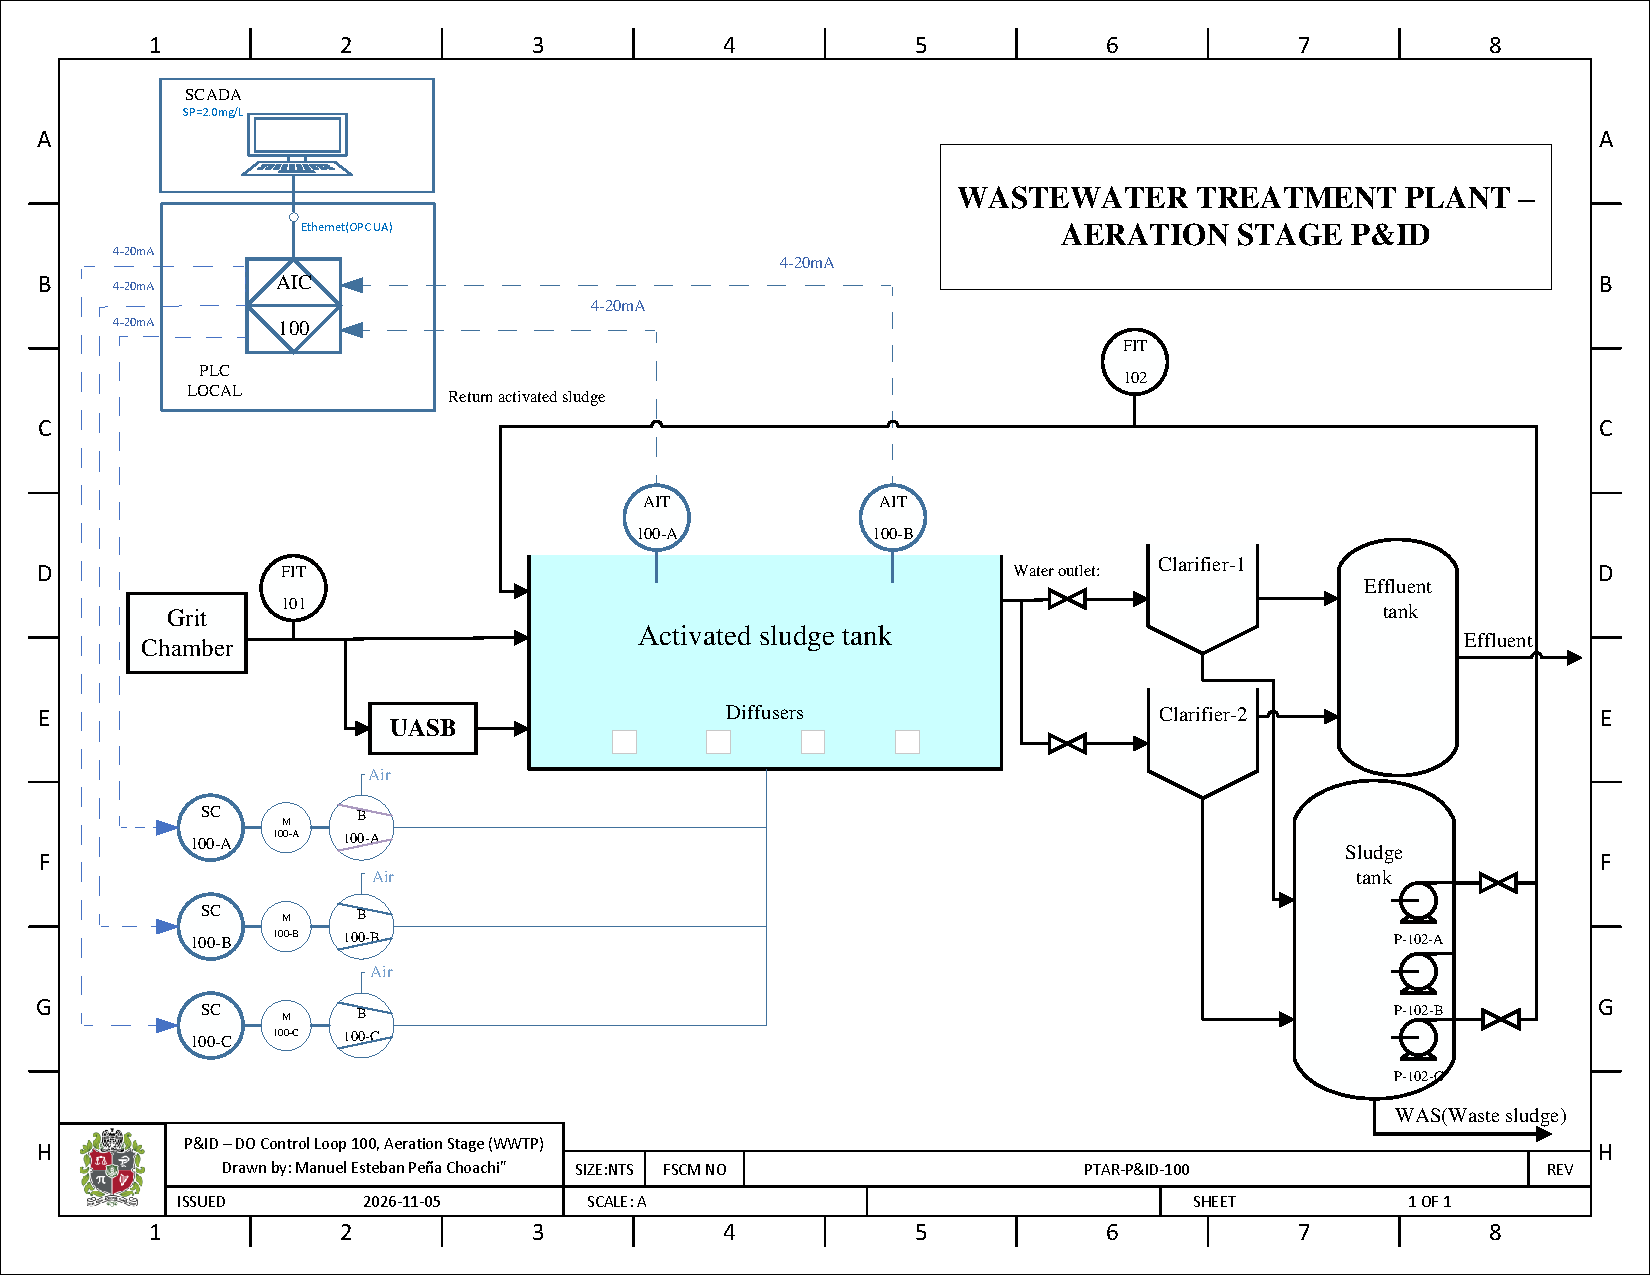
\includegraphics[width=\textwidth]{pid_ptar.pdf}
    \caption[P\&ID simplificado de la etapa de aireación]{P\&ID simplificado de la
    etapa de aireación según la simbología ISA-5.1.}
    \label{fig:pid_tikz}
\end{figure}

\subsection*{Etapas del proceso}

\begin{itemize}
  \item \textbf{Pretratamiento y desarenador.} El caudal de entrada pasa por
  rejillas y filtros continuos, que retiran los elementos más pesados, y por
  los desarenadores, que separan el líquido de la arena y otros sólidos.

  \item \textbf{Reparto del caudal.} A la salida del desarenador el caudal se
  divide en dos líneas: una va directamente al tanque de aireación y la
  otra al UASB.

  \item \textbf{UASB} (\emph{Upflow Anaerobic Sludge Blanket}). Es un reactor
  anaerobio que degrada la materia orgánica y produce biogás. De él salen tres
  corrientes: el biogás, un flujo líquido que entra al tanque de aireación (sin
  transmisor que lo mida) y un flujo sólido que va al tanque de lodos.

  \item \textbf{Tanque de aireación.} Es el reactor de lodos activados,
  donde la biomasa aerobia degrada la materia orgánica con el oxígeno que
  entregan los difusores ubicados en el fondo.

  \item \textbf{Sedimentadores o clarificadores.} Reciben la mezcla del
  tanque de aireación y separan el agua tratada de la biomasa, que se acumula
  en el fondo y se envía al tanque de lodos. El agua tratada se almacena y sale
  como efluente.


  \item \textbf{Recirculación de lodos (RAS).} Parte del lodo vuelve desde el
  tanque de lodos al tanque de aireación para mantener la concentración de
  biomasa.
\end{itemize}

\subsection*{Lazo 100: control de oxígeno disuelto}

Ahora bien, el lazo más importante es el 100, que constituye el control de
oxígeno disuelto. Sus componentes, en el orden en que viaja la señal, son:

\begin{itemize}
  \item \textbf{Transmisores de oxígeno AIT-100-A y AIT-100-B.} Miden la
  variable del proceso, es decir, el oxígeno disuelto a la entrada y a la
  salida del tanque de aireación, y envían una señal de 4--20~mA al PLC local.

  \item \textbf{PLC local (AIC-100).} Está en un tablero en campo, cerca del proceso.
  Convierte las señales de 4--20~mA a mg/L según la hoja técnica de los
  transmisores y calcula el promedio de las dos medidas de oxígeno. Seguido a
  esto, el controlador AIC-100 compara ese promedio con la referencia de 2,0~mg/L y
  calcula la señal de control $u$, que dentro del PLC se maneja como una
  consigna de 0 a 100~\% y se traduce a una señal de 4--20~mA para los
  variadores.

  \item \textbf{SCADA.} Registra el oxígeno disuelto y, desde él, el
  operador cambia la consigna, que llega al PLC por Ethernet.

  \item \textbf{Variadores SC-100-A/B/C.} Reciben la señal de control como
  4--20~mA y fijan la velocidad de los motores.

  \item \textbf{Sopladores B-100-A/B/C.} Accionados por sus motores, envían
  el aire de proceso.

  \item \textbf{Difusores.} Distribuyen el aire en el fondo del tanque de
  aireación, donde el oxígeno se transfiere al agua y cierra el lazo sobre la
  medida de los AIT.
\end{itemize}

La Figura~\ref{fig:lazo100_bloques} muestra el mismo lazo en bloques, en el orden en que
viaja la señal, antes de escribir cada bloque como una función de transferencia (Sección~\ref{sec:car_modelo}).

\begin{figure}[!htbp]
    \centering
    \resizebox{\textwidth}{!}{%
    \begin{tikzpicture}[>=Stealth, thick, font=\small,
        blq/.style={draw, thick, fill=white, align=center, minimum height=1.15cm, inner sep=4pt},
        suma/.style={draw, thick, circle, fill=white, minimum size=0.5cm, inner sep=0pt}]
        % ---- PLC local: controlador y promedio ----
        \draw[thin, dashed, gray!70!black, rounded corners=3pt] (1.1,-3.25) rectangle (3.7,1.05);
        \node[font=\footnotesize, gray!40!black, anchor=north west] at (1.15,1.02) {PLC local};
        % ---- camino directo: controlador, actuador y planta ----
        \node[suma] (s) at (0,0) {};
        \node[blq] (aic) at (2.4,0) {Controlador\\AIC-100};
        \node[blq] (sc) at (7.0,0) {Variadores\\SC-100-A/B/C};
        \node[blq] (sop) at (11.0,0) {Motores y\\sopladores};
        \node[blq] (dif) at (13.9,0) {Difusores};
        \node[blq, fill=cyan!8] (tq) at (17.2,0) {Tanque de\\aireación};
        \draw[->] (-1.6,0) -- node[above, align=center, font=\footnotesize] {consigna $r$\\(SCADA)} (s.west);
        \draw[->] (s.east) -- node[above, font=\footnotesize] {error} (aic.west);
        \draw[->] (aic.east) -- node[above, font=\footnotesize, pos=0.6] {$u$ [\%]} node[below, font=\footnotesize, pos=0.6] {4--20 mA} (sc.west);
        \draw[->] (sc.east) -- (sop.west);
        \draw[->] (sop.east) -- node[above, font=\footnotesize] {aire} (dif.west);
        \draw[->] (dif.east) -- node[above, font=\footnotesize] {oxígeno} (tq.west);
        \draw[->] (17.2,1.6) node[above, font=\footnotesize] {perturbaciones: caudales y carga} -- (tq.north);
        \draw[->] (tq.east) -- (19.9,0) node[above left, font=\footnotesize] {OD};
        \fill (19.2,0) circle (2pt);
        % ---- realimentacion: medida ----
        \node[blq] (ait) at (13.6,-2.4) {Transmisores\\AIT-100-A y AIT-100-B};
        \node[blq] (prom) at (2.4,-2.4) {Promedio de\\los sensores};
        \draw[->] (19.2,0) -- (19.2,-2.4) -- (ait.east);
        \draw[->] (13.6,-3.75) node[below, font=\footnotesize] {ruido de medida} -- (ait.south);
        \draw[->] (ait.west) -- node[above, font=\footnotesize] {4--20 mA} (prom.east);
        \draw[->] (prom.west) -- (0,-2.4) -- node[left, font=\footnotesize, pos=0.5] {OD medido $y$} (s.south);
        \node[font=\footnotesize] at ($(s.west)+(-0.2,-0.28)$) {$+$};
        \node[font=\footnotesize] at ($(s.south)+(0.28,-0.22)$) {$-$};
    \end{tikzpicture}}
    \caption[Lazo de control 100 en bloques]{Lazo de control 100 en diagrama de bloques.}
    \label{fig:lazo100_bloques}
\end{figure}

\subsection*{Lazos 101 y 102: caudales}

Al tanque de aireación llegan tres caudales: el directo del desarenador, el que
sale del UASB y la recirculación de lodos. Estos lazos solo miden los flujos de
líquido que entran al tanque, de modo que desde el punto de vista del control se
pueden ver como perturbaciones. Todos los caudales de la planta se registran en L/s.

\begin{itemize}
  \item \textbf{FIT-101.} Transmisor indicador de caudal a la salida del
  desarenador. Mide el caudal total antes del reparto.
  \item \textbf{FIT-102.} Transmisor indicador del caudal de recirculación de
  lodos (caudalímetro de 12~in), que mueven las bombas P-102-A, P-102-B y P-102-C.
  \item \textbf{Flujo del UASB.} No tiene transmisor, por lo que no se mide.
\end{itemize}


\section{Modelo dinámico}
\label{sec:car_modelo}

El modelo parte de un balance de masa de oxígeno disuelto sobre el tanque de
aireación, considerado como un reactor de mezcla completa. Se utilizaron como
guía las ecuaciones del BSM1 \cite{alex2008bsm1} y del ASM1
\cite{henze1987asm1}, adaptando las unidades a las que manejan los operarios de
la planta; en particular, el tiempo se expresa en horas, mientras que en el
BSM1 está en días.

\begin{equation}
\text{Acumulación}=\text{Entrada}-\text{Salida}+\text{Generación}-\text{Consumo}.
\end{equation}

Al tanque entran los tres caudales identificados en el P\&ID: el directo del
desarenador, el que sale del UASB y la recirculación de lodos ($i=1,2,3$). La
generación es la transferencia de oxígeno de los difusores, y el consumo es la
respiración de la biomasa. Así, el balance queda de la siguiente forma:

\begin{equation}
\frac{dS_O}{dt}=\frac{1}{V}\sum_{i=1}^3 Q_{in,i}\,S_{O_{in,i}}
-\frac{Q_{out}}{V}\,S_O+K_{La}\left(S^{*}_O-S_O\right)-r_z(S_O),
\label{eq:car_balance}
\end{equation}

con las variables de la Tabla~\ref{tab:car_variables}, y cada término tiene unidades de concentración
por unidad de tiempo:

\begin{equation}
\underbrace{\frac{dS_O}{dt}}_{\frac{\mathrm{mg}}{\mathrm{L}\cdot\mathrm{h}}}
=
\underbrace{\frac{1}{V}\sum_{i=1}^3 Q_{in,i}S_{O_{in,i}}}_{\frac{1}{\mathrm{L}}
\left(\frac{\mathrm{L}}{\mathrm{h}}\right)
\left(\frac{\mathrm{mg}}{\mathrm{L}}\right)
=
\frac{\mathrm{mg}}{\mathrm{L}\cdot\mathrm{h}}}
-
\underbrace{\frac{Q_{out}}{V}S_O}_{\left(\frac{\mathrm{L}/\mathrm{h}}{\mathrm{L}}\right)
\left(\frac{\mathrm{mg}}{\mathrm{L}}\right)
=
\frac{\mathrm{mg}}{\mathrm{L}\cdot\mathrm{h}}}
+
\underbrace{K_{La}(S^{*}_O-S_O)}_{\left(\frac{1}{\mathrm{h}}\right)
\left(\frac{\mathrm{mg}}{\mathrm{L}}\right)
=
\frac{\mathrm{mg}}{\mathrm{L}\cdot\mathrm{h}}}
-
\underbrace{r_z(S_O)}_{\frac{\mathrm{mg}}{\mathrm{L}\cdot\mathrm{h}}}.
\label{ecu:nonlineal}
\end{equation}

\begin{table}[H]
\centering
\caption{Variables del balance de oxígeno disuelto \eqref{eq:car_balance}.}
\label{tab:car_variables}
\renewcommand{\arraystretch}{1.2}
\small
\begin{tabular}{@{}l>{\raggedright\arraybackslash}p{9.2cm}l@{}}
\toprule
\textbf{Variable} & \textbf{Descripción} & \textbf{Unidades} \\
\midrule
$S_O$ & Oxígeno disuelto en el tanque de aireación & mg/L \\
$S_{O_{in,i}}$ & Oxígeno disuelto de cada caudal de entrada & mg/L \\
$Q_{in,i}$ & Caudales de entrada: desarenador, UASB y recirculación de lodos ($i = 1, 2, 3$) & L/h \\
$Q_{out}$ & Caudal de salida del tanque & L/h \\
$V$ & Volumen del tanque de aireación & L \\
$K_{La}$ & Coeficiente de transferencia de oxígeno de los difusores & h$^{-1}$ \\
$S^{*}_O$ & Concentración de saturación de oxígeno & mg/L \\
$r_z$ & Consumo de oxígeno por la respiración de la biomasa & mg/(L$\cdot$h) \\
$t$ & Tiempo & h \\
\bottomrule
\end{tabular}
\end{table}

El consumo de oxígeno $r_z$ se toma del ASM1, como en el BSM1: es el término $r_{Z,5}$ del
tanque 5 cambiado de signo, $r_z = -r_{Z,5}$, con $r_{Z,5}$ dado por \eqref{eq:intro_rz} en la
Sección~\ref{subsec:intro_od} \cite{henze1987asm1,alex2008bsm1}.


Ahora bien, la variable que realmente se manipula no es $K_{La}$ sino la
consigna $u$ que el PLC envía a los variadores. Si se considera que el
coeficiente de transferencia es proporcional a esa señal, quedaría de la
siguiente forma:

\begin{equation}
K_{La} = k_\alpha\, u , \qquad u \in [0,100]~\%,
\end{equation}

donde $k_\alpha$ es una constante de proporcionalidad que, en el rango de
operación, se puede estimar como

\begin{equation}
k_\alpha = \frac{K_{La_{max}}-K_{La_{min}}}{100-0},
\qquad
\left[k_\alpha\right] = \left[\frac{\mathrm{h}^{-1}}{\%}\right].
\end{equation}

Esta ganancia agrupa toda la cadena de actuación, desde la señal del PLC hasta
la transferencia de oxígeno en los difusores, como se descompone en la
Tabla~\ref{tab:gain_decomposition}. Se aclara que esta relación es solo una
aproximación, y se utiliza para entender las suposiciones del modelo
simplificado y las discrepancias que van a existir entre este y el
comportamiento real de la planta.

\begin{table}[!htbp]
\centering
\caption{Descomposición de la ganancia $k_\alpha$ a lo largo de la cadena de
actuación.}
\label{tab:gain_decomposition}
\begin{tabular}{cll}
\toprule
\textbf{Etapa} & \textbf{Conversión} & \textbf{Ganancia} \\
\midrule
1. PLC          & 0--100~\% $\to$ 4--20\,mA          & $k_{\mathrm{PLC}} = 0{,}16$\,mA/\% \\
2. Variador / motor  & 4--20\,mA $\to$ 0--3000\,rpm  & $k_{\mathrm{VFD}} = 187{,}5$\,rpm/mA \\
3. Soplador     & $n \to Q_{\mathrm{aire}}$            & $k_Q = Q_{\mathrm{aire}}^{\max}/n^{\max}$ \\
4. Aireación    & $Q_{\mathrm{aire}} \to K_{La}$      & $k_{K_{La}}$ \\
\midrule[\heavyrulewidth]
\multicolumn{2}{l}{\textbf{Ganancia total} $k_\alpha = K_{La}/u$}
                & $k_\alpha = k_{K_{La}}\, k_Q\, k_{\mathrm{VFD}}\, k_{\mathrm{PLC}}$ \\
\bottomrule
\end{tabular}
\end{table}

Sustituyendo $K_{La}=k_\alpha u$ en el balance \eqref{eq:car_balance}, la
dinámica queda en forma afín respecto a la entrada $u$:

\begin{equation}
\dot S_O
=
\underbrace{
\frac{1}{V}\sum_{i=1}^3 Q_{in,i}S_{O_{in,i}}
-\frac{Q_{out}}{V}S_O
-r_z(S_O)
}_{f(S_O,t)}
+
u\,
\underbrace{
k_\alpha\left(S^{*}_O-S_O\right)
}_{g(S_O,t)},
\end{equation}

es decir,

\begin{equation}
\dot S_O = f(S_O,t) + g(S_O,t)\,u .
\label{eq:car_afin}
\end{equation}

Por ende, el sistema no es lineal: la ganancia de entrada $g$ depende del
propio oxígeno disuelto; es decir, la entrada $u$ aparece multiplicada por
una variable de estado del sistema. Este tipo de problema entra en el campo de
los sistemas no lineales, y si bien se podría resolver con técnicas más
complejas, en este caso se optó por
validar un enfoque al estilo del ADRC. Este consiste en agrupar toda la
dinámica que difiere de un integrador puro dentro de una perturbación total
$\bar{\xi}$, y dejar fuera solo una ganancia de entrada constante $\overline{b_0}$:

\begin{equation}
    \dot{y} = \bar{\xi} + \overline{b_0}\, K_{La},
\end{equation}

Ahora bien, si se agrega el término $\overline{b_0}\, K_{La}$, es necesario
restarlo dentro de la perturbación total para que la ecuación no cambie,
quedando de la siguiente forma:

\begin{equation}
\bar{\xi}
=
\frac{1}{V}\sum_{i=1}^3 Q_{in,i}S_{O_{in,i}}
-\frac{Q_{out}}{V}S_O
-r_z(S_O)+K_{La}\left(S^{*}_O-S_O\right)-\overline{b_0}\, K_{La}.
\end{equation}

Sustituyendo de nuevo $K_{La} = k_\alpha u$:


\begin{equation}
\bar{\xi}
=
\frac{1}{V}\sum_{i=1}^3 Q_{in,i}S_{O_{in,i}}
-\frac{Q_{out}}{V}S_O
-r_z(S_O)
+ {\color{red}{k_\alpha u}} \left(S^{*}_O-S_O\right)
-\overline{b_0}\, {\color{red}{k_\alpha u}},
\label{ecu:disturbance}
\end{equation}

y definiendo $b_0 = \overline{b_0}\, k_\alpha$, con unidades

\begin{equation}
\left[b_0\right]=\left[\frac{\mathrm{mg}}{\mathrm{L}}\right] \cdot \left[\frac{\mathrm{h}^{-1}}{\%}\right]
= \left[\frac{\mathrm{mg}}{\mathrm{L}\cdot\mathrm{h}\cdot\%}\right],
\end{equation}

se llega a la forma canónica del ADRC de primer orden, en la que cada término
tiene unidades consistentes para este sistema:

\begin{equation}
\underbrace{\dot{y}}_{\left[\frac{\mathrm{mg}}{\mathrm{L}\cdot\mathrm{h}}\right]}
=
\underbrace{\bar{\xi}}_{\left[\frac{\mathrm{mg}}{\mathrm{L}\cdot\mathrm{h}}\right]}
+
\underbrace{b_0}_{\left[\frac{\mathrm{mg}}{\mathrm{L}\cdot\mathrm{h}\cdot\%}\right]}
\cdot
\underbrace{u}_{[\%]} .
\label{eq:car_canonica}
\end{equation}

Ahora bien, en la práctica $b_0$ no se calcula a partir de los parámetros del
ASM1, que no se miden en la planta, sino que se obtiene de un modelo de primer
orden identificado con los datos. Ese modelo, con retardo $\theta$, es

\begin{equation}
G(s)=\frac{Y(s)}{U(s)}
=
\frac{k_{dc}}{\tau s+1}\,e^{-\theta s}.
\label{eq:car_foptd}
\end{equation}

Para el desarrollo que sigue se toma $\theta=0$, lo que simplifica el diseño
y permite ver con claridad la relación entre la planta y la perturbación total.
La simplificación es razonable porque el retardo, que se acota entre 0 y
60~s (Sección~\ref{sec:ident_retardo}), es pequeño frente a la constante de
tiempo, $\theta/\tau \leq 0{,}06$; su efecto se retoma al acotar el ancho
de banda del observador. Sin el retardo, y con una perturbación $\varepsilon(t)$ a la entrada, en las
mismas unidades de $u$, la planta \eqref{eq:car_foptd} en el tiempo es
\begin{equation}
\tau\,\dot{y}(t) + y(t) = k_{dc}\bigl(u(t) + \varepsilon(t)\bigr)
\quad\Longrightarrow\quad
\dot{y}(t) = b_0\left(u(t) + \varepsilon(t) - \frac{y(t)}{k_{dc}}\right),
\qquad b_0 = \frac{k_{dc}}{\tau} .
\end{equation}
La dinámica que sobra de la planta, el término $-y/k_{dc}$, hace parte de la perturbacion. Es decir, parte de la dinámica de la planta queda embebida dentro de la
perturbación total:
\begin{equation}
\dot{y}(t) = b_0\bigl(u(t) + \bar{\varepsilon}(t)\bigr),
\qquad
\bar{\varepsilon}(t) = \varepsilon(t) - \frac{y(t)}{k_{dc}},
\label{eq:planta_eps_bar}
\end{equation}
y la planta queda como un integrador puro. Si la perturbación se lleva al lado de la salida,
$\bar{\xi}(t) = b_0\,\bar{\varepsilon}(t)$, la ganancia de entrada que necesita el ADRC queda determinada
por los dos parámetros que se identifican en la planta,

\begin{equation}
b_0=\frac{k_{dc}}{\tau},
\qquad
\dot{y}(t)=\bar{\xi}(t) + b_0\, u(t),
\label{eq:car_b0}
\end{equation}

que es precisamente la forma del ADRC \eqref{eq:car_canonica}. En este caso,
la perturbación total abarca todos los términos mostrados en la
ecuación~\eqref{ecu:disturbance}: los caudales de entrada y de salida (es
importante mencionar que el caudal de salida se mantiene igual al de entrada,
de modo que el volumen del tanque es constante), la parte de la dinámica que
depende de la entrada y que no queda en $b_0$, el consumo de oxígeno por la
respiración biológica y las incertidumbres propias de algunos parámetros de la
planta. Las secciones siguientes se dedican a estimar $k_{dc}$, $\tau$ y
$\theta$ a partir del histórico de la planta, para obtener la ganancia $b_0$,
estimar la perturbación total y cuantificar el efecto que tiene cada
perturbación en la señal de control.

% ============================================================================
%  Caracterización a partir de los datos de planta
%  Figuras: figuras/ident_*.pdf, exportadas de
%  Datos/analisis/analisis_dinamica_limpio.ipynb
% ============================================================================
\section{Caracterización a partir de los datos de planta}
\label{sec:ident}

Esta sección reúne la caracterización del lazo de oxígeno hecha sobre los datos reales de la PTAR, que
vienen de dos fuentes. La primera es el historiador del SCADA, que guarda cada minuto el oxígeno disuelto
(OD) de los tres módulos y la potencia consumida por la aireación de M2 y M3, y cada hora los caudales,
niveles y presiones; con M2 y M3 se hacen la identificación por ventanas ARX, los caudales y la
perturbación total. La segunda son las trazas del PLC ctrlX del ensayo del 12 de marzo de 2026 en M1, que
no tiene medidor de potencia: muestreadas a 50~ms, son el único registro donde aparece directamente la
consigna $u$ que el PLC manda al variador, y de ellas salen el retardo, el ruido del sensor y la
comparación entre el SCADA y el PLC.

Como los tres módulos son idénticos en proceso, y la consigna de 0 a 100~\%
enviada por el PLC a los variadores no quedó en el histórico del SCADA, en M2 y
M3 se toma la potencia en porcentaje de plena carga,
$u = 100\,P/P_{\max}$, como si fuera la misma señal de control. $P_{\max}$ es una aproximación de
la plena carga y no el máximo del registro: se toma un valor cercano al percentil 99 de la potencia
registrada con el soplador encendido, $P_{\max} = 106{,}3$~kW en M2 y $110{,}1$~kW en M3. Con los dos
sopladores encendidos la potencia consumida no siempre es la misma, y en algunos casos pasa de ese
valor (Figura~\ref{fig:ident_segundo_soplador}); ahí $u$ supera el $100~\%$. Aun así, se deja este
valor en todo el trabajo, porque los $K$ y $\bo$ identificados están referidos a él. La diferencia entre la potencia y la señal de control, debida a la
cadena variador--motor--soplador y no exactamente lineal, no se modela por
separado: queda incluida en la perturbación total $\bar{\xi}$, igual que el
error al elegir $\bo$ (Secciones~\ref{sec:ident_arx} y~\ref{sec:car_modelo}).
El observador del ADRC la estima y la compensa junto con el resto de lo que el
modelo no representa.

% ----------------------------------------------------------------------------
\subsection{Línea temporal: el régimen de operación día a día}
\label{sec:ident_mapa}

Para saber qué datos se pueden utilizar para entender el sistema, cada día de
cada módulo se clasificó como PID en automático o manual. La clasificación se
hace a partir del error de seguimiento y de cuántas veces el OD cruza la
referencia, de cuánto se aleja el OD por encima de ella y de si el soplador
modula o está fijo.

La Figura~\ref{fig:ident_mapa} muestra el resultado. Ahora bien, los
días manuales son los que se usan para identificar la planta, y los de PID para
medir el desempeño del controlador actual y ver los problemas que presenta.

\begin{figure}[!htbp]
    \centering
    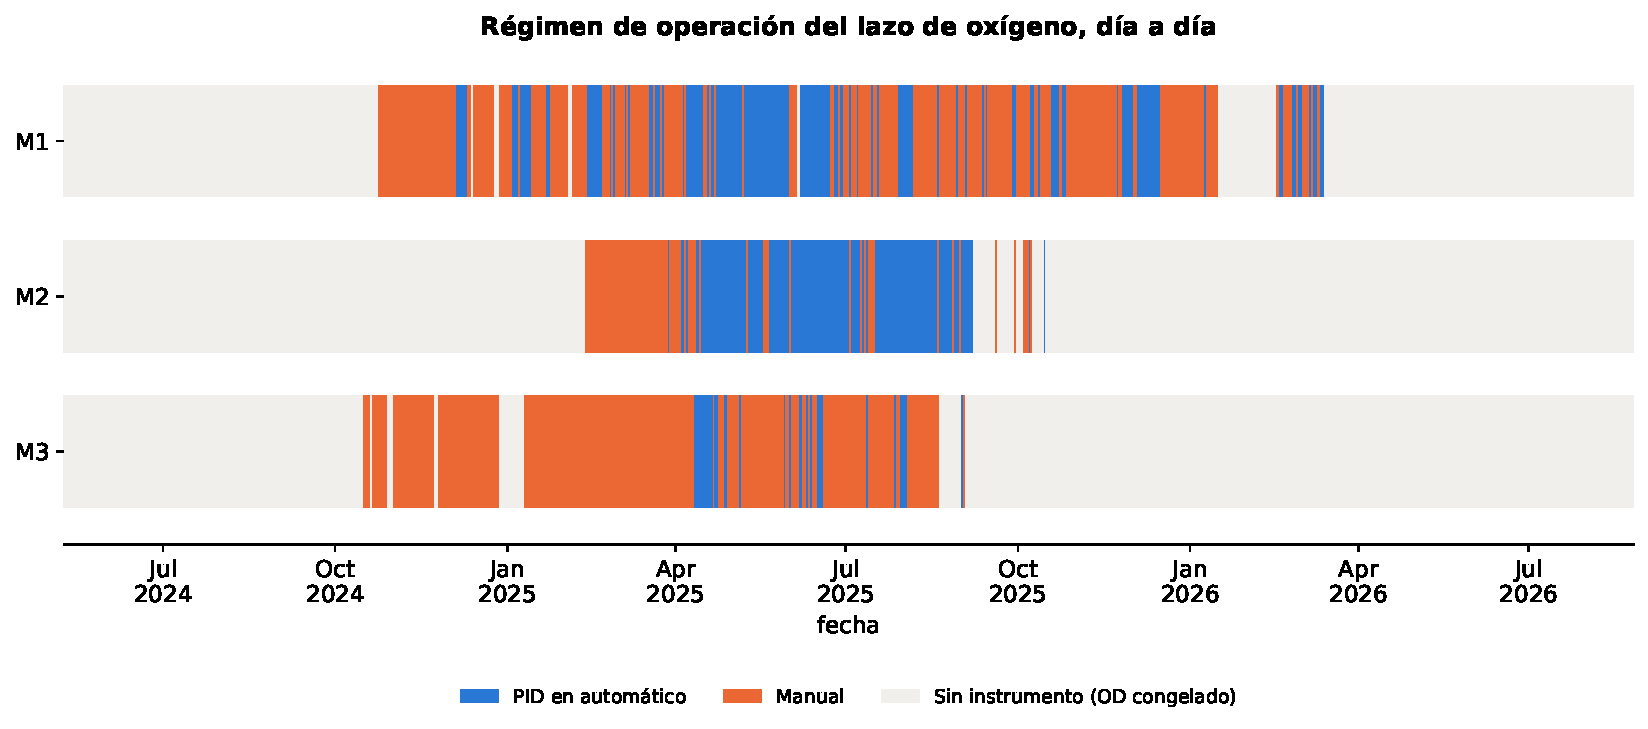
\includegraphics[width=\linewidth]{ident_02_mapa_operacion.pdf}
    \caption[Régimen de operación día a día]{Régimen de operación del lazo de
    oxígeno día a día en los tres módulos. Azul: PID en automático; naranja:
    manual; gris: sensor congelado.}
    \label{fig:ident_mapa}
\end{figure}


% ----------------------------------------------------------------------------
\subsection{Funcionamiento en lazo cerrado con PID}
\label{sec:ident_pid}

La referencia está fija en 2,0~mg/L durante todo el registro, así que no hay
escalones de referencia. Lo equivalente son los arranques del soplador bajo
PID: el lazo parte del OD en el suelo y tiene que llevarlo a la referencia.

La Figura~\ref{fig:ident_pid_arranques} muestra arranques de M2 donde la
variable del proceso (el OD) llega a la referencia sin oscilaciones, con un
sobreimpulso pequeño, de 5,1 y 7,7~\%. Como el arranque parte de cero, el cambio de consigna es la propia referencia,
$r = 2{,}0$~mg/L, y el sobreimpulso queda en porcentaje de ella. En
cambio, en la Figura~\ref{fig:ident_pid_oscilatorio}, en
otras fechas, se ve un comportamiento subamortiguado en los dos módulos: un
sobreimpulso de 44~\% en M2 y de 91~\% en M3, y una serie de picos con
envolvente decreciente hasta que llega al estacionario.

\begin{figure}[!htbp]
    \centering
    \subfloat[Los dos mejores arranques en M2: el OD llega a la referencia sin
    oscilar.]{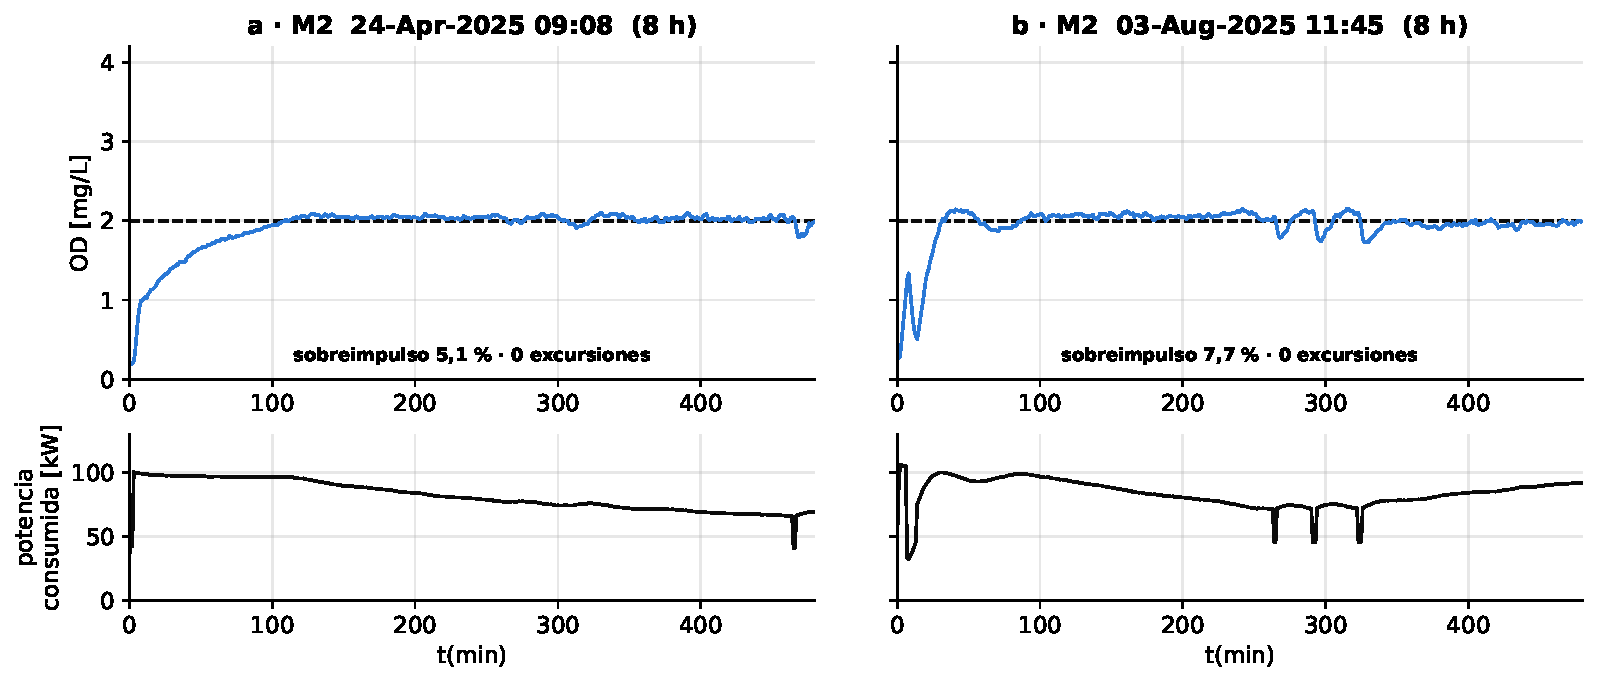
\includegraphics[width=\linewidth]{ident_13_pid_arranques.pdf}%
    \label{fig:ident_pid_arranques}}\\
    \subfloat[Arranques en su versión oscilatoria, en M2 y M3: subamortiguados
    pero convergentes; los círculos marcan los picos sucesivos sobre la
    referencia.]{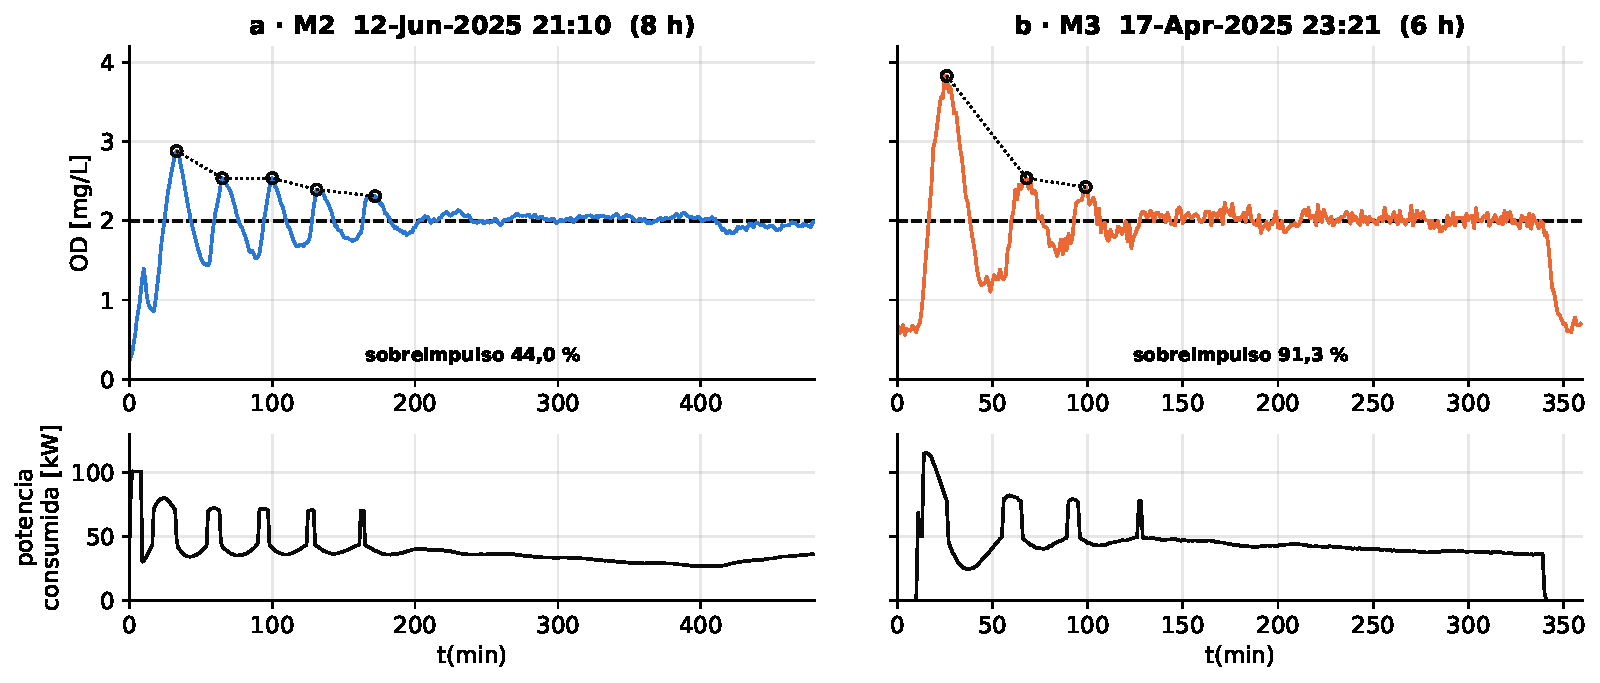
\includegraphics[width=\linewidth]{ident_14_pid_oscilatorio.pdf}%
    \label{fig:ident_pid_oscilatorio}}
    \caption[Arranques del PID actual]{Arranques del PID actual en la planta.
    La línea discontinua es la referencia de 2,0~mg/L; abajo de cada panel, la
    potencia consumida en kW.}
    \label{fig:ident_pid}
\end{figure}

Por lo tanto, cuando el sistema tiene condiciones diferentes, a
veces llega a la referencia limpiamente y otras veces oscila. Esto es coherente
con lo que se muestra más adelante en la identificación: la ganancia de la planta cambia de una
ventana a otra (Sección~\ref{sec:ident_arx}), aunque desde el
enfoque del ADRC la ganancia se mantiene constante y lo que cambia es la
perturbación total del sistema. Ahora bien, en algunos casos el OD está en el
suelo y la planta casi no responde; por consiguiente, el PID acumula acción
integral. Cuando el sistema se libera y tiene las condiciones para elevar el
oxígeno, el control puede estar ya saturado por la acumulación de la acción
integral, lo que produce sobreimpulso y algunas oscilaciones, y en los casos en
que no se tenga un sistema de anti-\emph{windup}, el lazo puede volverse
inestable. Por ello, en capítulos posteriores se utilizará para el GPI un
esquema de anti-\emph{windup} que ayude con el manejo de la saturación.



% ----------------------------------------------------------------------------
\subsection{Escalones de soplador en lazo abierto}
\label{sec:ident_escalones}

En los días de operación manual los operarios encienden y apagan el soplador a mano, con escalones de
distinto tamaño y duración: sin proponérselo, es un ensayo de identificación en lazo abierto. En esos
escalones el OD tarda más en subir que en bajar, una asimetría que un modelo lineal de primer orden no
puede reproducir. Además, la ganancia no es única: cambia de un escalón a otro y de un módulo a otro,
porque las perturbaciones y las no linealidades ponen a cada uno en una región distinta de su dinámica,
no porque los modelos sean distintos. Un ejemplo es el mismo escalón de M2 en dos días
(Figura~\ref{fig:ident_escalon_3mgL}): con casi la misma potencia y partiendo del mismo suelo, el
16-abr-2025 el OD asienta en 3,06~mg/L y el 26-feb-2025 en 1,93~mg/L. Las dos curvas tienen casi la
misma constante de tiempo; lo que cambia es la ganancia, 1,7 veces mayor el primer día. Es la misma
planta, cuya ganancia cambia con las perturbaciones.

\begin{figure}[!htbp]
    \centering
    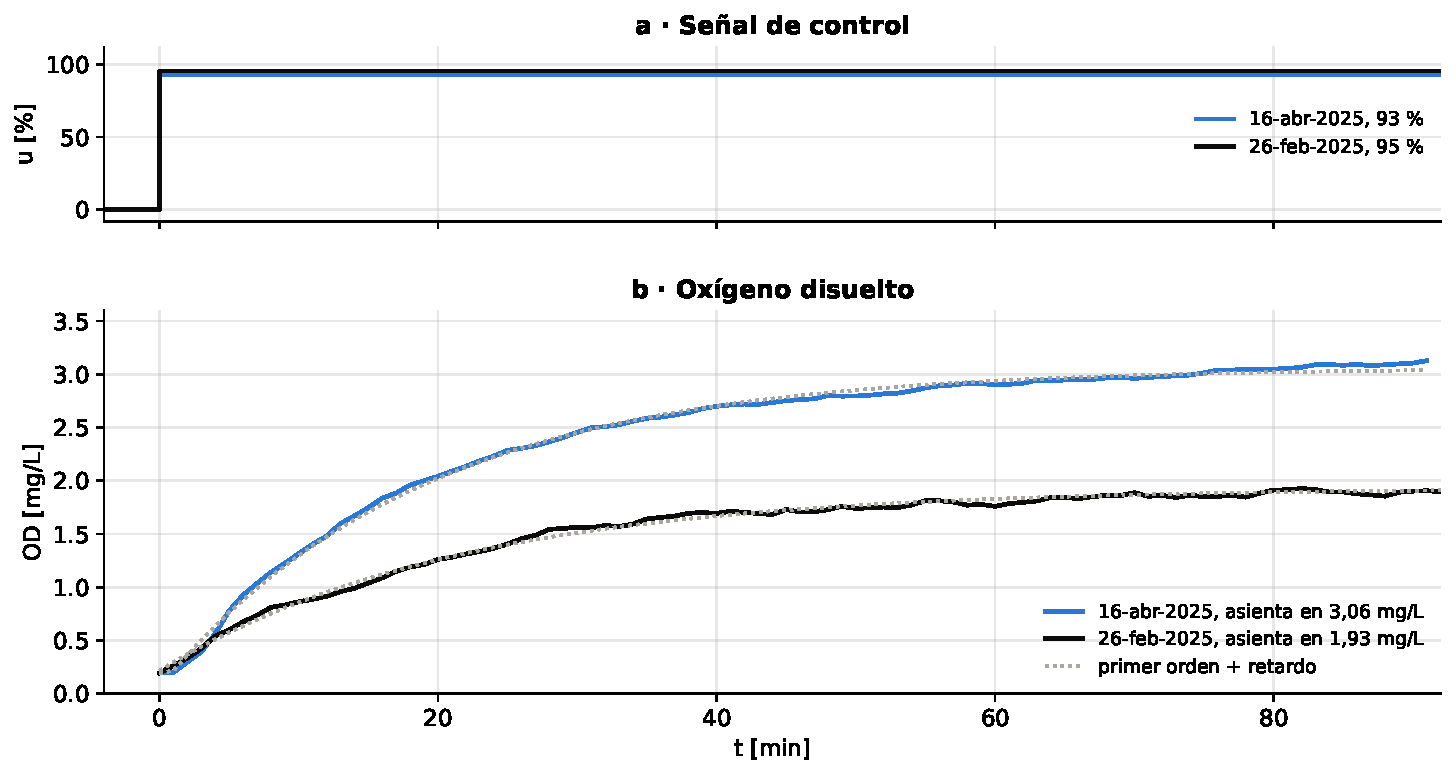
\includegraphics[width=0.85\linewidth]{ident_16_escalon_3mgL.pdf}
    \caption[El mismo escalón de M2 en dos días]{El mismo escalón de M2 en dos días, el 16-abr-2025 y
    el 26-feb-2025: (a) señal de control en porcentaje y (b) OD, que asienta en 3,06 y 1,93~mg/L. La
    línea punteada es el ajuste de primer orden con retardo.}
    \label{fig:ident_escalon_3mgL}
\end{figure}

\paragraph{Un escalón alrededor de la referencia.} Casi todos los escalones
anteriores van de soplador apagado a plena carga, y el OD recorre de casi 0 a
más de 4~mg/L. En M3 hay una identificación en el punto de operación, realizada el 13-jun-2025
(Figura~\ref{fig:ident_escalon_ref}). Con 40~kW el OD se asienta en
1,08~mg/L; a las 04:16 la potencia sube a 60~kW ($\Delta u = 18{,}1$~\% de
plena carga) y el OD llega a 2,50~mg/L.
\begin{equation*}
K = \frac{\Delta y}{\Delta u} = \frac{2{,}50 - 1{,}08}{18{,}1}
  = 0{,}079~\mathrm{mg/(L\cdot\%)},
\end{equation*}

\begin{figure}[H]
    \centering
    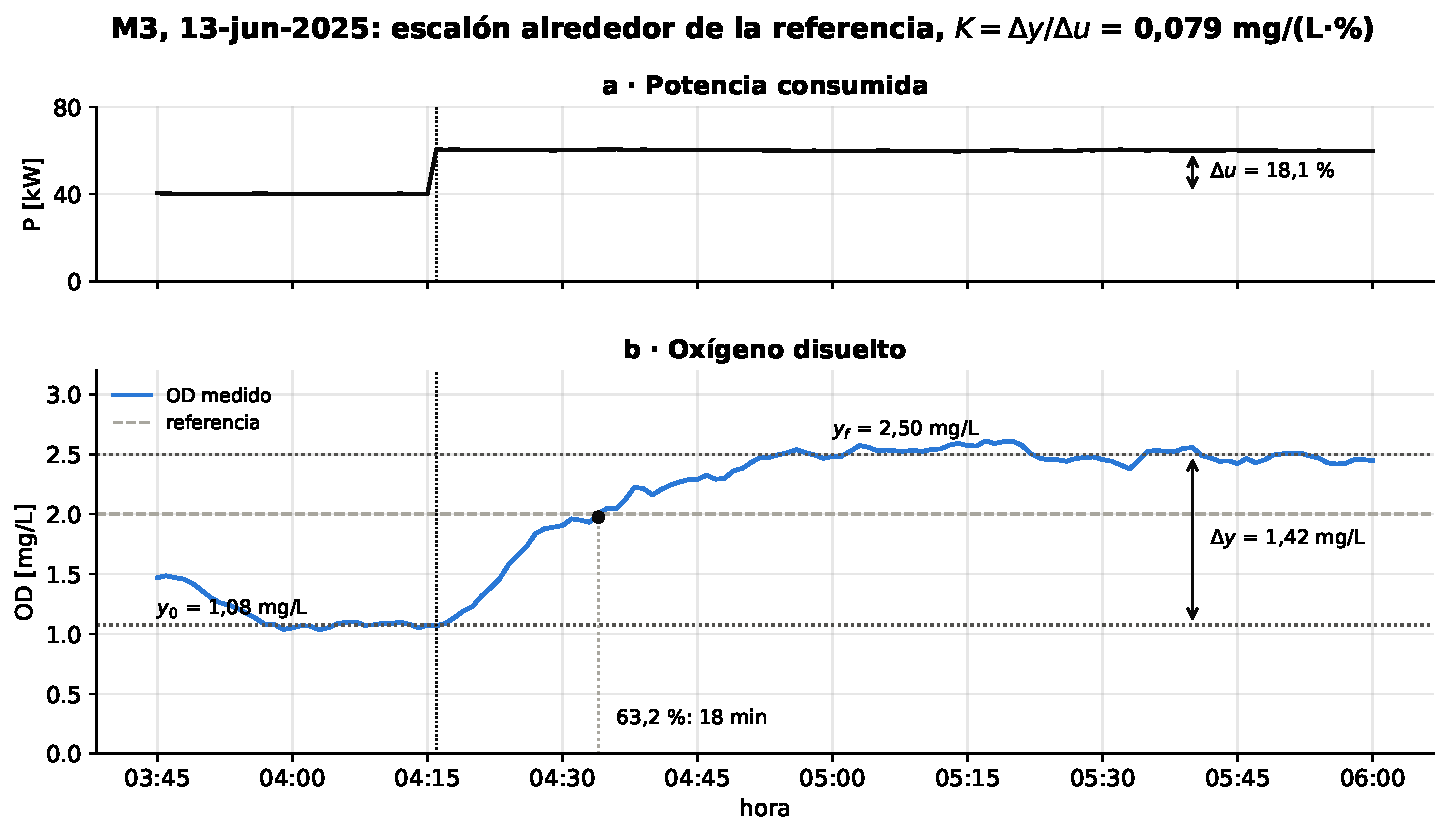
\includegraphics[width=0.75\linewidth]{ident_21_escalon_referencia.pdf}
    \caption[Escalón alrededor de la referencia]{Escalón de M3 del 13-jun-2025
    alrededor de la referencia: (a) la potencia pasa de 40 a 60~kW a las 04:16 y
    (b) el OD va de 1,08 a 2,50~mg/L, con $K = \Delta y/\Delta u = 0{,}079$~mg/(L$\cdot$\%).}
    \label{fig:ident_escalon_ref}
\end{figure}

% ----------------------------------------------------------------------------
\subsection{Segundo soplador}
\label{sec:ident_segundo_soplador}

La planta se operaba con una sola señal de control de 0 a $100~\%$ repartida entre los dos
sopladores: el primer $50~\%$ de la señal lleva un soplador hasta su máximo y el otro $50~\%$ es para
el segundo. En la Figura~\ref{fig:ident_segundo_soplador}, con un soplador el OD se queda casi quieto,
y al entrar el segundo sube rápido; cuando se apaga, vuelve a bajar. Por eso se decidió conectar los
dos sopladores a la misma señal de control de 0 a $100~\%$, sin fraccionarla. Aun así, el ADRC debería
poder asimilar la entrada del segundo soplador: mientras el sistema no llegue a la referencia actúa el
anti-\emph{windup}, y cuando entra el segundo soplador, el exceso de potencia que aporta se toma como una
perturbación y el sistema llega a la referencia. Como anotación, aunque el sistema está diseñado para 3 sopladores, solo
se tienen en funcionamiento dos para las fechas de las pruebas.

\begin{figure}[H]
    \centering
    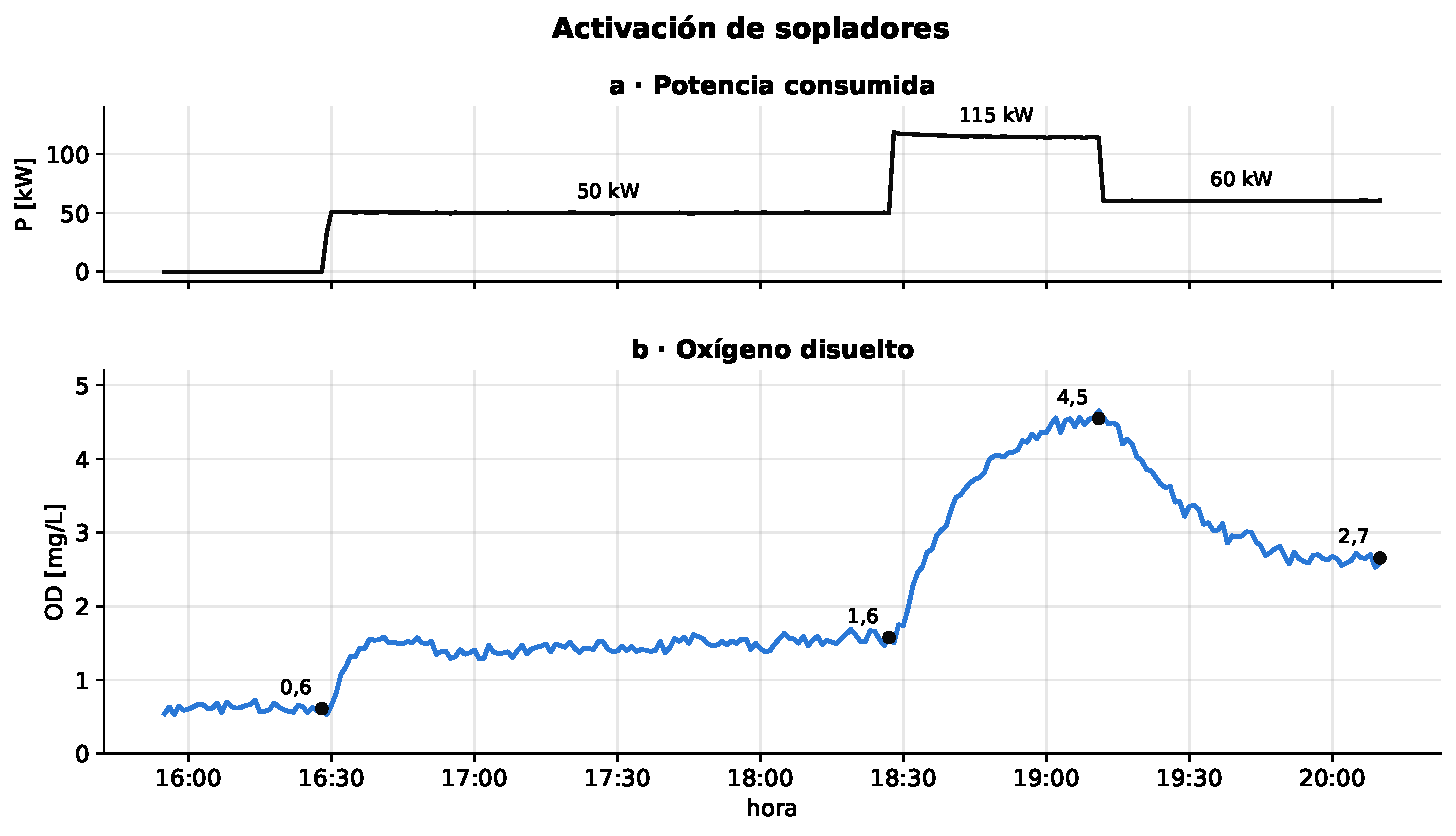
\includegraphics[width=0.85\linewidth]{ident_22_segundo_soplador.pdf}
    \caption[Entrada del segundo soplador en M3]{M3 el 26-abr-2025: (a) potencia consumida y (b) OD,
    con el valor que alcanza al final de cada cambio de potencia: apagado, un soplador a 50~kW, los dos a
    115~kW y de nuevo uno a 60~kW.}
    \label{fig:ident_segundo_soplador}
\end{figure}

% ----------------------------------------------------------------------------
\subsection{Retardo}
\label{sec:ident_retardo}

El SCADA, a 1~min, no puede resolver un retardo de menos de un minuto. El único
escalón que sí lo resuelve es el registrado por el PLC a 50~ms
(Figura~\ref{fig:ident_retardo}). La imagen muestra un retardo aproximado de
$\theta = 50$~s, y el OD sale de su ruido a los $\approx$ 58~s. A simple vista, el OD empieza a subir hacia los 50~s. Por
ende, para el diseño se considera un retardo entre 0 y 60~s, con ideal de 50~s, que abarca el espectro completo de $\theta$, y en
simulación se valida el controlador con estas variaciones del retardo.

\begin{figure}[H]
    \centering
    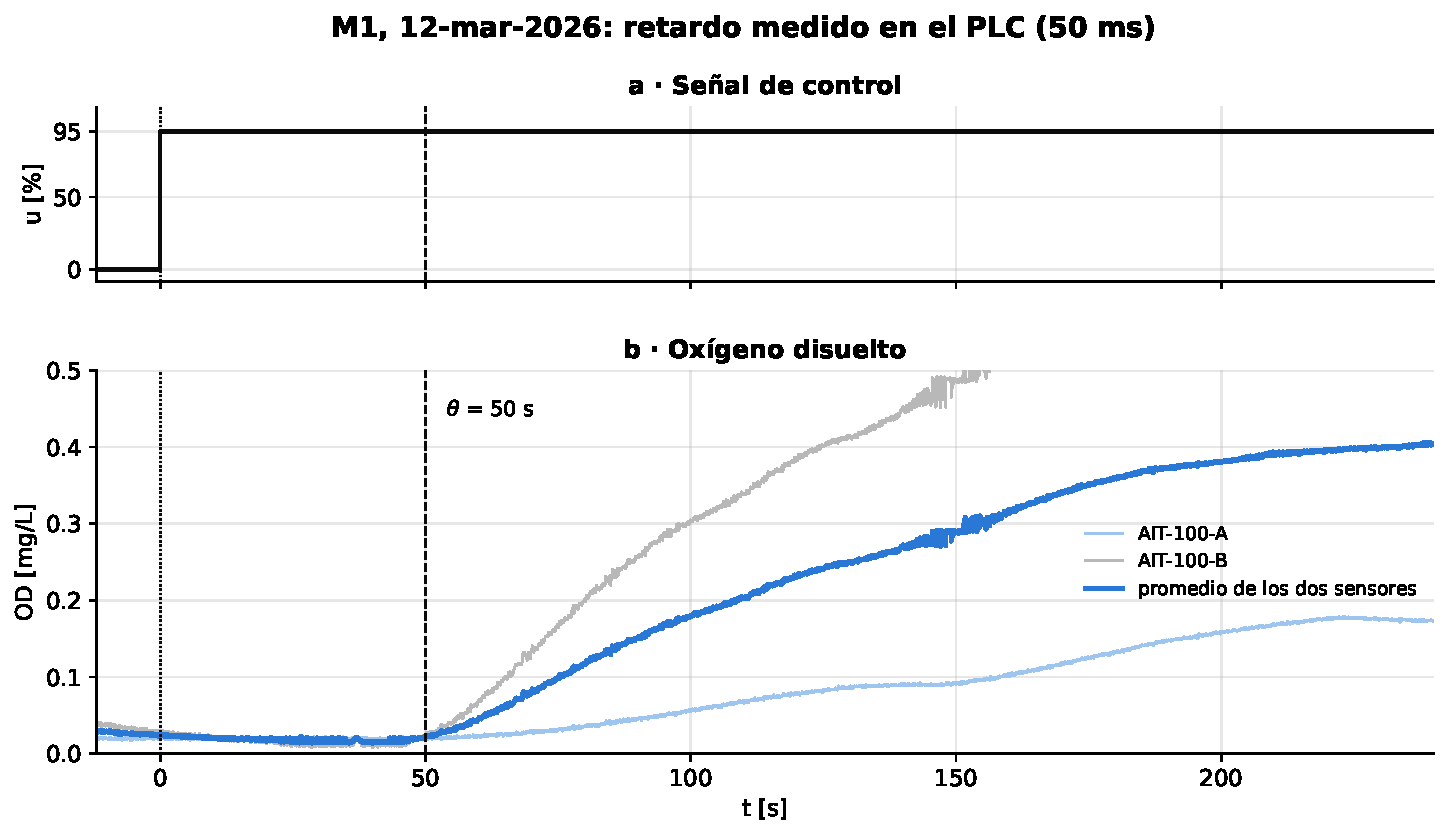
\includegraphics[width=0.85\linewidth]{ident_10_retardo_M1.pdf}
    \caption[Retardo medido en M1]{Primeros 4~min del escalón del
    12-mar-2026 en M1, registrado por el PLC ctrlX a 50~ms: (a) señal de control
    $u$ y (b) OD. La línea discontinua marca el retardo observado del sistema (50~s).}
    \label{fig:ident_retardo}
\end{figure}

% ----------------------------------------------------------------------------
\subsection{Rango de variación de $\tau$ y $K$}
\label{sec:ident_arx}

Sobre los días de lazo abierto se ajusta, en ventanas de 3~h, un modelo de
primer orden en tiempo discreto. Se utiliza una identificación ARX
(autorregresiva con entrada exógena), la más simple posible: un ARX(1,1) de
primer orden con término constante, estimado por mínimos cuadrados:
\begin{equation}
y[k+1] = \varphi\, y[k] + \gamma\, u[k] + \delta ,
\end{equation}
con $y$ el OD (oxígeno disuelto) y $u$ la señal de control en porcentaje,
obtenida a partir de los datos de potencia medidos. De sus coeficientes salen
$\tau = -T_s/\ln\varphi$, $K = \gamma/(1-\varphi)$ y $\bo = K/\tau$.

La Figura~\ref{fig:ident_pulso} muestra una ventana con su respectiva
identificación ante un escalón del soplador. Un solo par $\tau$, $K$ reproduce
el arranque y el estacionario, pero el OD real sube más lento de lo que cae,
mientras que el modelo tarda lo mismo en ambos sentidos; es decir, el modelo
promedia la dinámica de subida y la de bajada. Esa asimetría se mide sobre todos
los escalones en la Sección~\ref{sec:ident_validacion}.

\begin{figure}[!htbp]
    \centering
    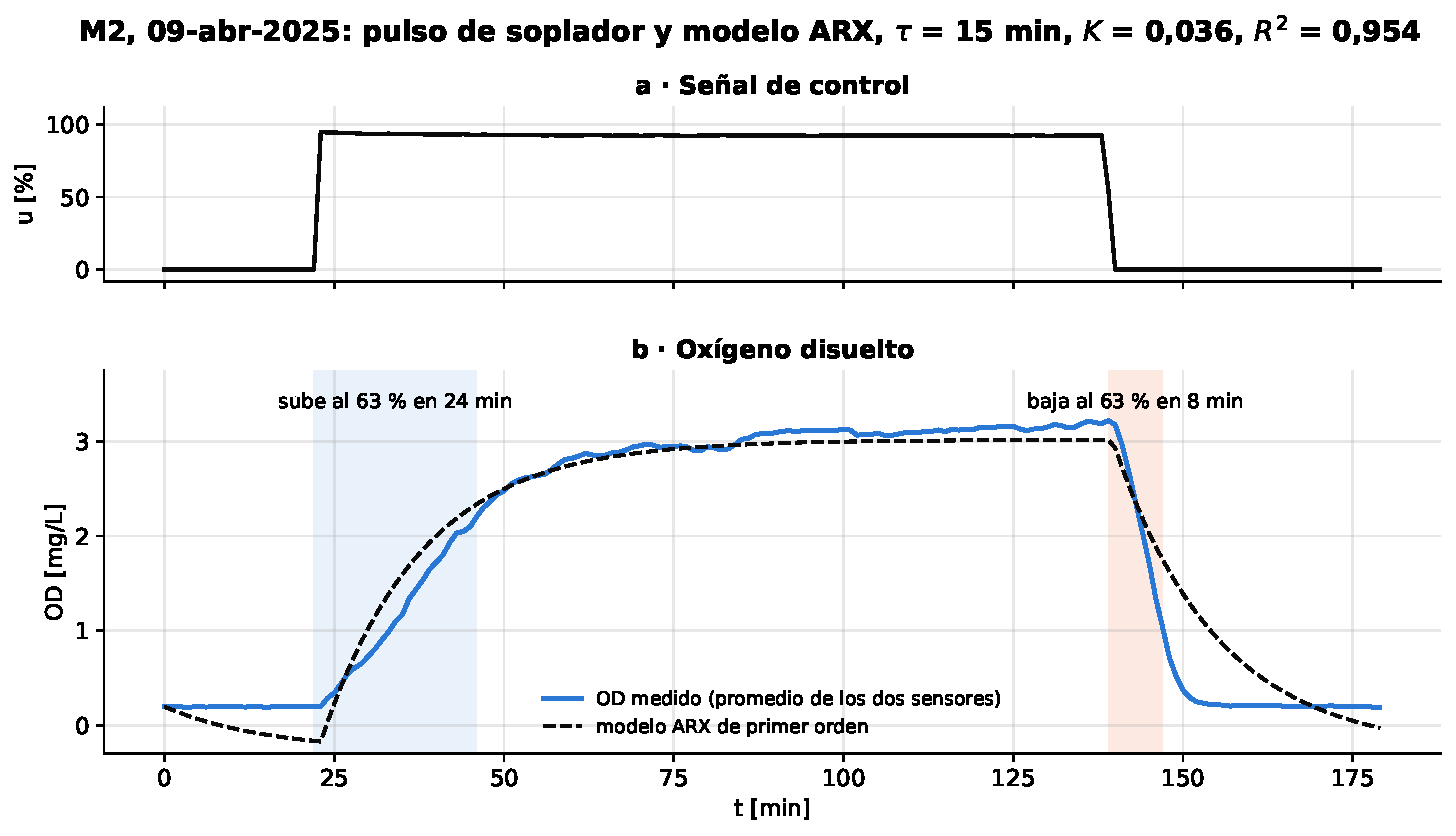
\includegraphics[width=0.85\linewidth]{ident_03_pulso_arx.pdf}
    \caption[Identificación ARX sobre un pulso]{Ajuste ARX sobre una ventana de
    3~h de M2 en lazo abierto y validación por simulación libre. Las franjas
    marcan el tiempo al 63~\% medido en el dato al subir y al bajar.}
    \label{fig:ident_pulso}
\end{figure}

En la literatura, cuando se diseña un controlador lineal para un
sistema no lineal, lo usual es linealizar alrededor de un punto de operación
con escalones pequeños cerca de ese punto. En este trabajo el diseño también se
hizo en un punto de operación, el de 2~mg/L
(Sección~\ref{sec:ident_planta_diseno}), pero la identificación se hizo con
todos los escalones recolectados, en todo el rango de operación de la planta y
del actuador, para conocer cuánto varían la ganancia y la constante de tiempo
del sistema, y verificar que el ADRC funciona en todo ese rango sin cambiar los
parámetros del controlador.

Para eso, el ajuste se repite en ventanas deslizantes de 3~h con paso de 1~h,
descartando las ventanas sin excitación, con $R^2 < 0{,}5$ o con $\tau$ fuera
de 1--300~min. Las distribuciones que quedan son anchas
(Figura~\ref{fig:ident_pob}): la identificación promedia la subida y la bajada,
y además la ganancia cambia de una ventana a otra. Por eso la
Tabla~\ref{tab:ident_arx} reporta medianas y, como rango, el intercuartílico, es
decir, el intervalo donde cae la mitad central de las ventanas.

\begin{table}[!htbp]
\centering
\caption{Ventanas ARX de lazo abierto: mediana y, entre paréntesis, rango
intercuartílico.}
\label{tab:ident_arx}
\footnotesize
\begin{tabular}{lcc}
\toprule
 & \textbf{M2} & \textbf{M3} \\
\midrule
Ventanas & 1225 & 1822 \\
$\tau$ [min] & 16,9 (11 -- 26) & 24,4 (15 -- 40) \\
$K$ [mg/(L$\cdot$\%)] & 0,0201 (0,0077 -- 0,0342) & 0,0649 (0,0212 -- 0,109) \\
$\bo$ [mg/(L$\cdot$h$\cdot$\%)] & 0,059 (0,0335 -- 0,107) & 0,149 (0,0816 -- 0,224) \\
\bottomrule
\end{tabular}
\end{table}

\subsection{Validación del modelo}
\label{sec:ident_validacion}

Con el ARX se obtuvo un modelo lineal de primer orden en cada ventana. Ahora
bien, falta responder si ese modelo realmente abarca la mayor parte de la
información del fenómeno. Para eso se comparan los parámetros del ARX con los
de los escalones medidos directamente en la planta, primero como poblaciones y
después escalón por escalón.

Los escalones de soplador son la referencia más directa del comportamiento real: en cada uno se
ve cuánto tarda el OD en responder y cuánto llega a cambiar, por separado para
las subidas y para las bajadas. Se toman los 532 escalones que pasan un filtro
estricto ($|\Delta u| \geq 20$~\%, al menos 90~min de duración,
$R^2 \geq 0{,}90$, respuesta asentada y $|\Delta y| \geq 0{,}30$~mg/L), y cada
uno se ajusta con un primer orden. Si el modelo ARX representa bien la planta, sus
parámetros deberían parecerse a los de los escalones.

La Figura~\ref{fig:ident_pob} pone las tres poblaciones juntas: las ventanas
ARX, los escalones que suben y los escalones que bajan. Como hay muchas más
ventanas ARX que escalones, cada histograma se normaliza como densidad, con área
1, para poder comparar las poblaciones, y el eje horizontal está en escala
logarítmica.

\begin{figure}[!htbp]
    \centering
    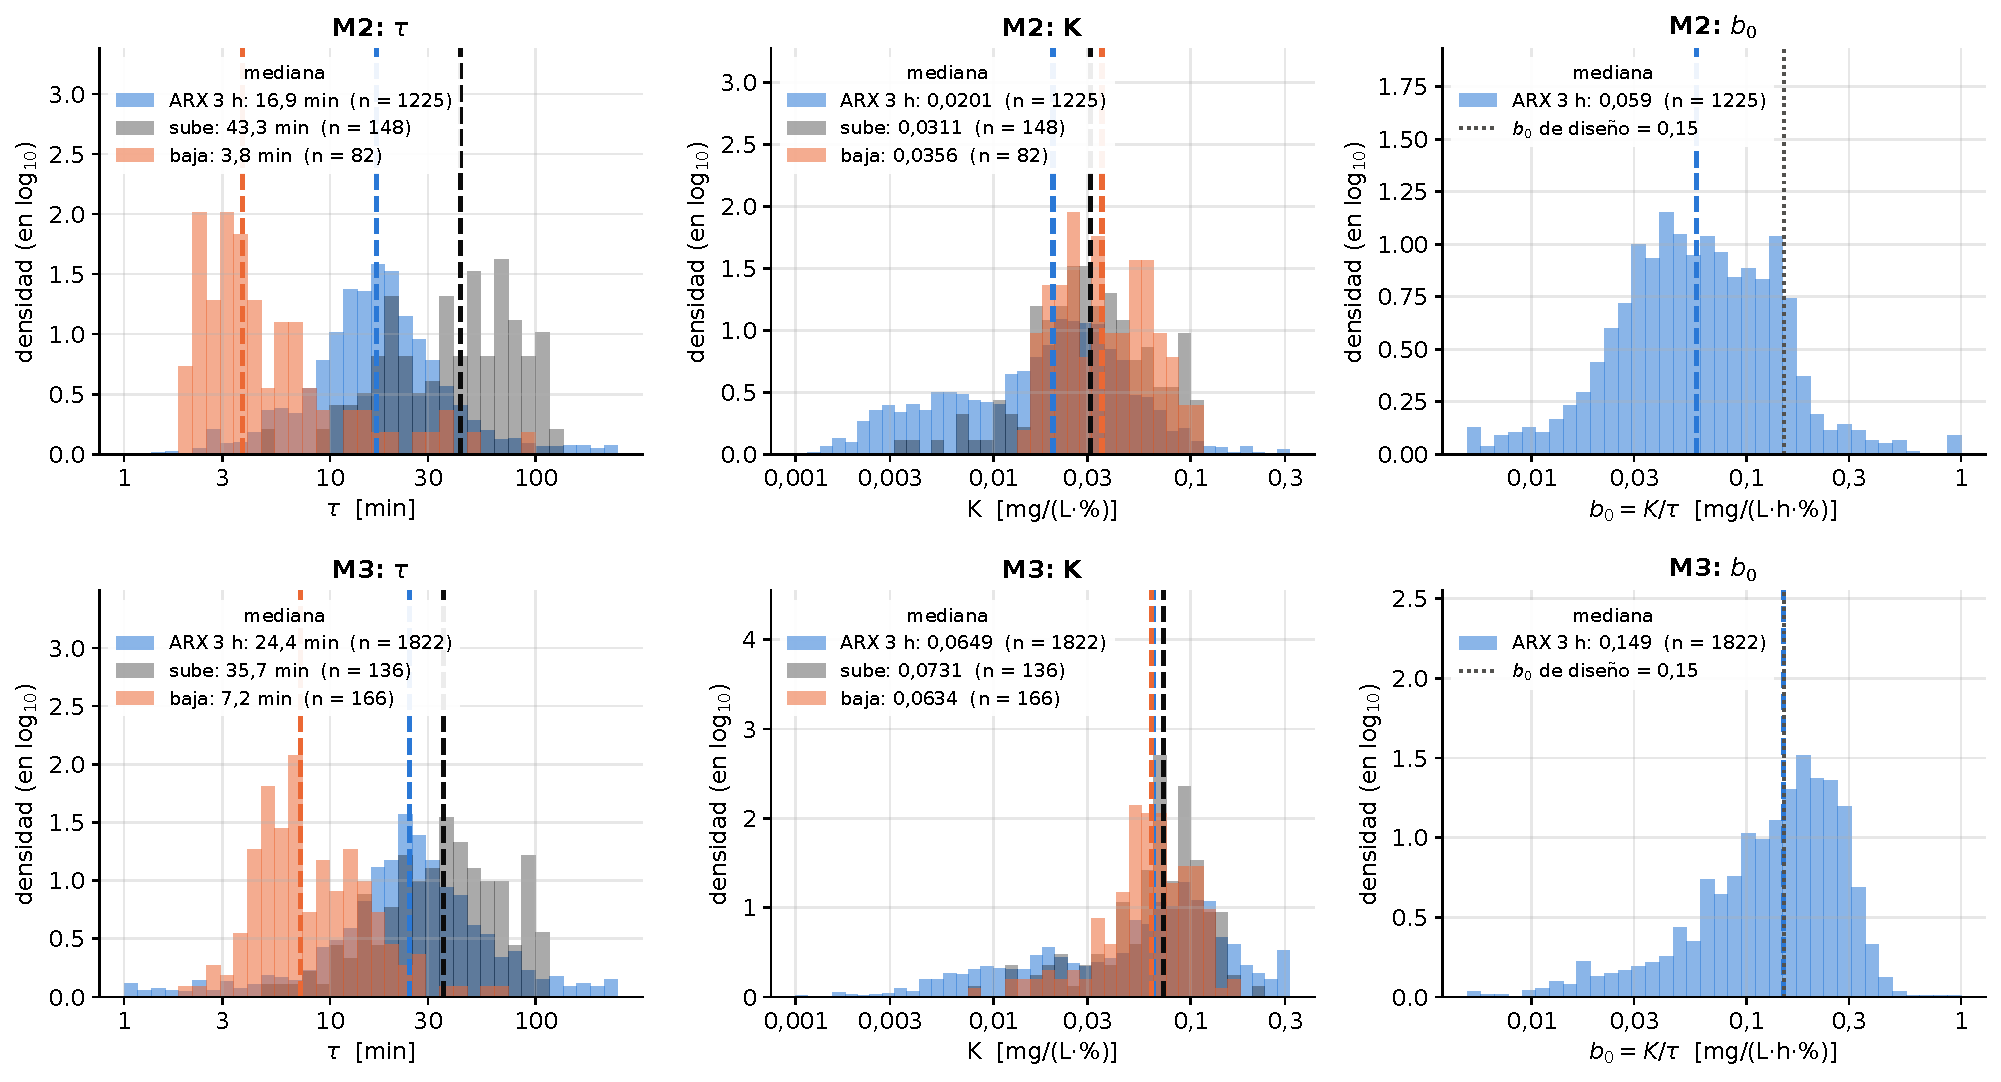
\includegraphics[width=\linewidth]{ident_05_poblaciones_tau_K.pdf}
    \caption[Poblaciones de $\tau$, $K$ y $\bo$ en M2 y M3]{Las tres poblaciones
    de la constante de tiempo (izquierda), de la ganancia estática (centro) y de
    la ganancia de entrada $\bo = K/\tau$ (derecha) en M2 (arriba) y M3 (abajo):
    ventanas ARX de 3~h, escalones que suben y escalones que bajan (en $\bo$,
    solo las ventanas ARX). Histogramas en densidad, con el eje horizontal en escala logarítmica; las
    líneas discontinuas son las medianas, la punteada de la derecha es el $\bo$
    de diseño (0,15) y los valores fuera del eje se acumulan en las barras de los
    extremos.}
    \label{fig:ident_pob}
\end{figure}

En la constante de tiempo (columna izquierda) las tres poblaciones no coinciden, como se esperaba por
la asimetría de la Sección~\ref{sec:ident_escalones}: los escalones que suben son lentos, los que bajan
rápidos, y el ARX, que ajusta un solo $\tau$ en ventanas con subidas y bajadas, queda en un valor
intermedio. En la ganancia $K$, en cambio, los escalones que suben y los que bajan dan valores
parecidos: la asimetría es solo dinámica. Por ende, el modelo ARX captura bien el orden de magnitud de
la ganancia y una constante de tiempo promedio, pero no la asimetría; esa parte la agrupa el observador
del ADRC dentro de la perturbación total, y así el controlador la tolera sin conmutar parámetros.

\paragraph{Comparación escalón por escalón.} Los histogramas comparan
poblaciones completas, pero no dicen si el ARX acierta en cada caso. Para
eso, sobre cada escalón limpio se ajustó también el ARX, y se comparó con dos valores que se leen directamente
en el dato, sin ajustar ningún modelo: el tiempo que tarda el OD en recorrer el
63~\% del salto ($t_{63}:\tau$) y la ganancia real, $\Delta y/\Delta u$. La
Figura~\ref{fig:ident_validacion} muestra el resultado: cada punto es un
escalón, el eje horizontal es el valor medido y el vertical el del ARX, y la
diagonal punteada indica que los dos coinciden.

\begin{figure}[!htbp]
    \centering
    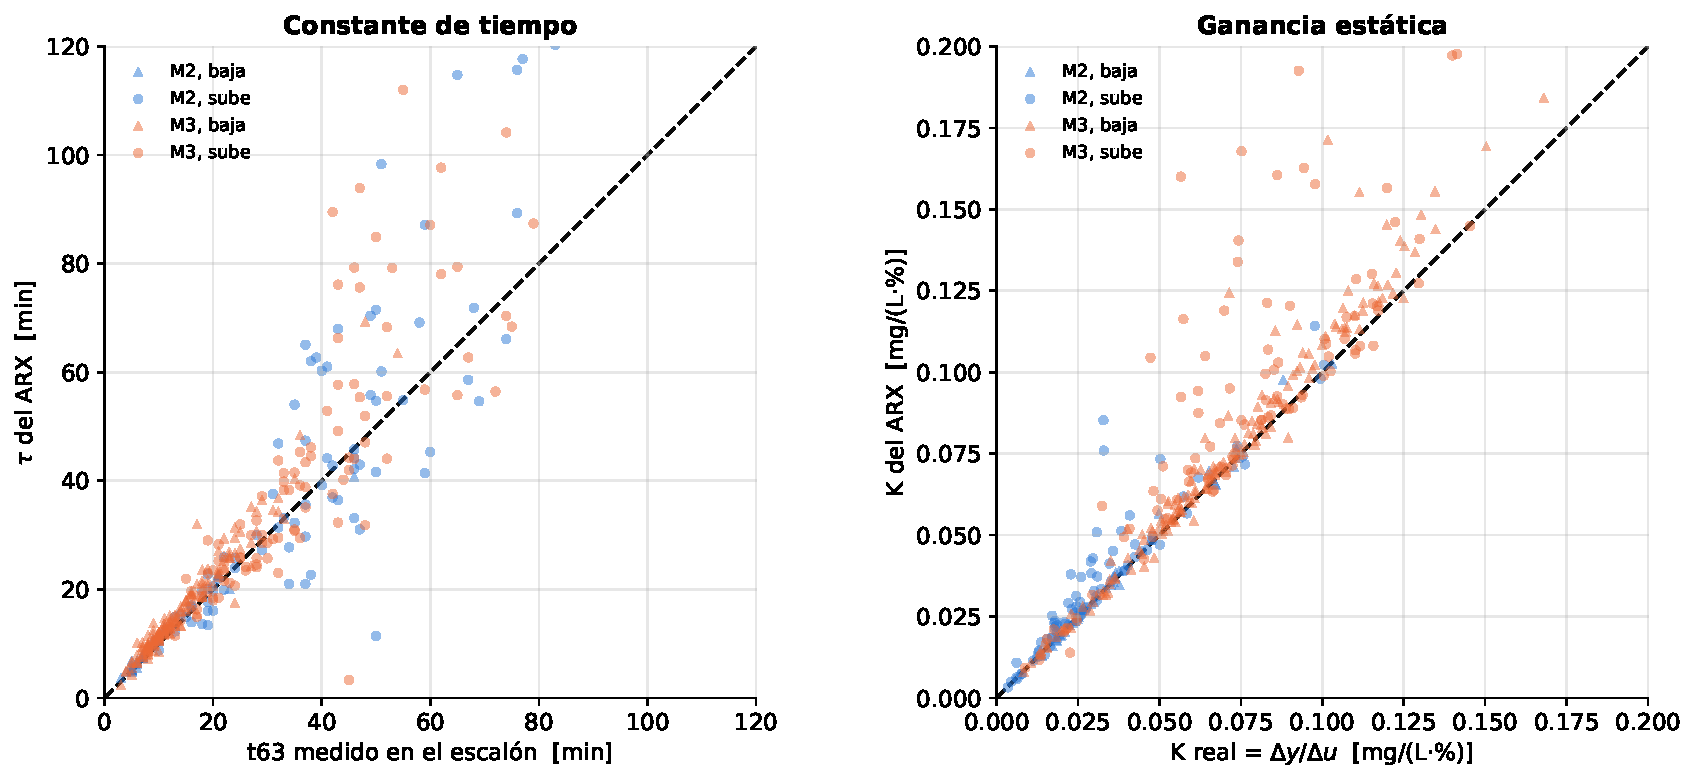
\includegraphics[width=\linewidth]{ident_10_validacion_arx.pdf}
    \caption[Validación del ARX escalón por escalón]{Validación del ARX escalón
    por escalón. Izquierda: constante de tiempo del ARX frente al tiempo al
    63~\% medido en el dato. Derecha: ganancia del ARX frente a la ganancia
    real $\Delta y/\Delta u$. Círculos: escalones que suben; triángulos:
    escalones que bajan. La diagonal es la igualdad.}
    \label{fig:ident_validacion}
\end{figure}

En la ganancia los puntos caen sobre la diagonal en todo el rango, tanto en M2
como en M3 y tanto al subir como al bajar. En la constante de tiempo también siguen la
diagonal; las bajadas, que son rápidas, quedan muy pegadas a ella, y las
subidas lentas se dispersan más, porque al arrancar desde un OD muy bajo la
respuesta no es una exponencial limpia. Por ende, cuando el ARX mira un solo
escalón reproduce lo que se mide en la planta, y esto valida que el espectro de
ganancias que entrega la identificación (Sección~\ref{sec:ident_arx}) es válido para la planta.



% ----------------------------------------------------------------------------
\subsection{Perfil diario de los caudales}
\label{sec:ident_caudales}

Los caudales de M2 se toman del historiador del SCADA, que registra cada hora,
en L/s, el caudal de entrada a la salida del desarenador (FIT-101) y el de
recirculación de lodos (FIT-102). Cada registro es una muestra instantánea del
caudal en ese momento. La
Figura~\ref{fig:ident_caudales_perfil}a muestra un día completo de los dos
caudales, tal como los guarda el SCADA. La recirculación, en cambio, solo se enciende durante periodos cortos. Aun así, el controlador debe poder
rechazar esos cambios y, si llegara a saturarse mientras la bomba está
encendida, mantener la saturación controlada hasta que se apague.


Ahora bien, el caudal cambia de un día para otro y varía aleatoriamente. No es predecible; lo que se puede
medir es el rango en el que los operarios lo tratan de mantener.
En la Figura~\ref{fig:ident_caudales_perfil}b, siete días seguidos se
superponen al ciclo diario (la media de los datos medidos en cada hora durante los días de referencia); Lo que cada registro se aparta del ciclo tiene una desviación estándar
robusta de 13,6~L/s. Es decir, el caudal de entrada es sobre todo aleatorio, con un ciclo
diario débil que está alrededor de un valor de DC de aproximadamente 34~L/s. Por ende, la perturbación, que depende de los caudales de entrada
según la ecuación~\eqref{ecu:disturbance} que se modela en la sección
siguiente tiene la misma estructura: un nivel, un ciclo diario débil y una parte
aleatoria de mayor magnitud.

\begin{figure}[H]
    \centering
    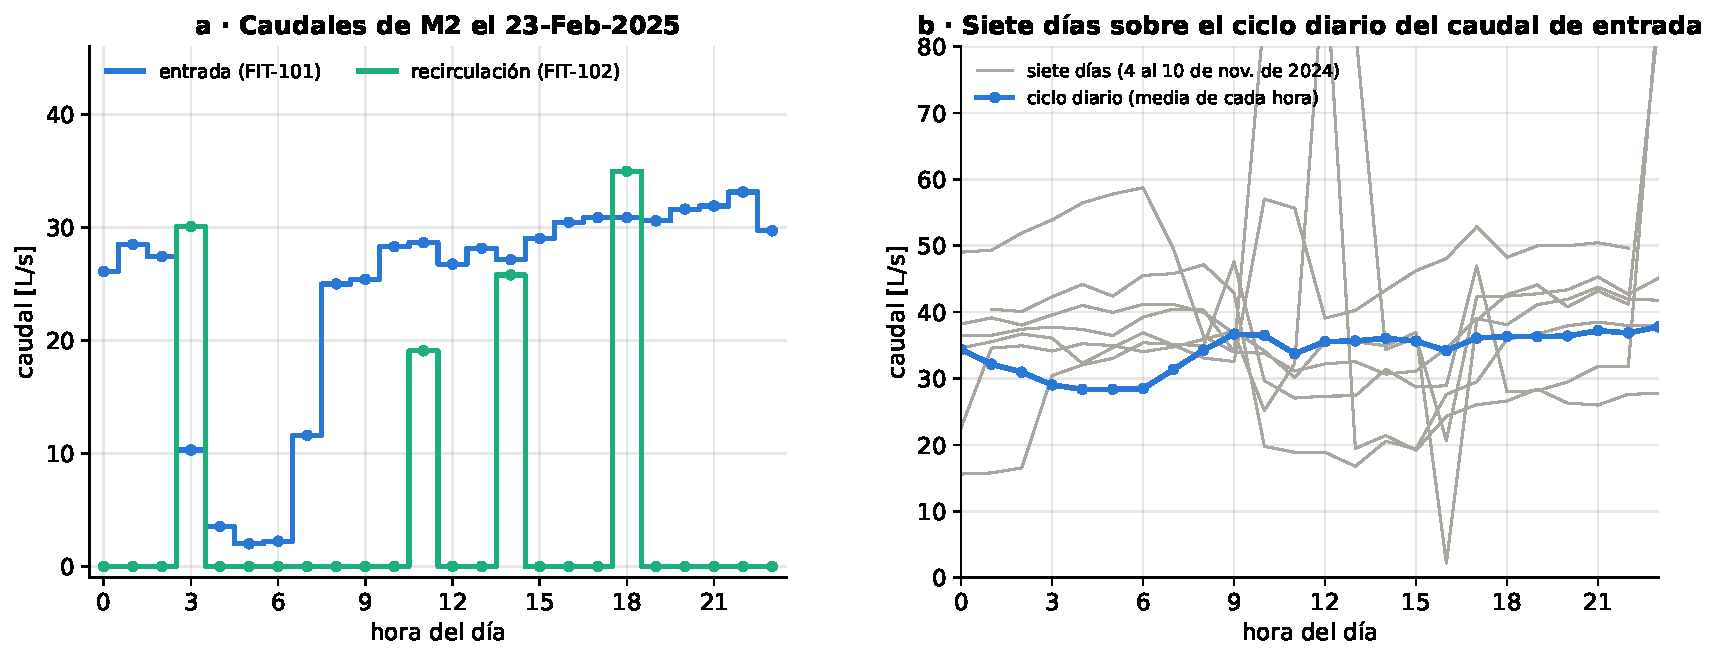
\includegraphics[width=\linewidth]{ident_11_caudales_perfil.pdf}
    \caption[Caudales de M2]{Caudales de M2: (a) entrada (FIT-101) y
    recirculación (FIT-102) el 23 de febrero de 2025, con un registro por hora
    del SCADA; (b) caudal de entrada del 4 al 10 de noviembre de 2024 (en gris)
    sobre su ciclo diario (media de cada hora).}
    \label{fig:ident_caudales_perfil}
\end{figure}

La Figura~\ref{fig:ident_recirculacion}a muestra lo que pasa cuando se enciende
la recirculación con el PID en la consigna. Antes de la bomba, el PID sostenía
los 2~mg/L con el soplador a poco más de un tercio de su potencia; al
encenderse, sube la potencia hasta el máximo del soplador y, aun así, el OD baja
hasta 0,84~mg/L. Así que el lazo queda saturado mientras la bomba está
encendida. Cuando se apaga, el OD tarda varias horas en volver a la consigna y
solo entonces la potencia empieza a bajar. 

No siempre satura. En la Figura~\ref{fig:ident_recirculacion}b, con el
sistema en estacionario en la consigna, se enciende la bomba y el PID sube la
señal de control unos 12 puntos; el OD apenas se aparta de la consigna, y al
apagarse la bomba la señal vuelve casi al nivel de antes. Como el caudal de
entrada se mantuvo casi constante mientras la bomba estuvo encendida, ese cambio
se debe a la recirculación. Este cambio de unos 12 puntos es el que se usa más adelante
para elegir la perturbación de entrada de las simulaciones, $\varepsilon = -15~\%$
(Sección~\ref{subsec:caso_simulacion}): del mismo orden que la medida, y algo mayor.

\begin{figure}[H]
    \centering
    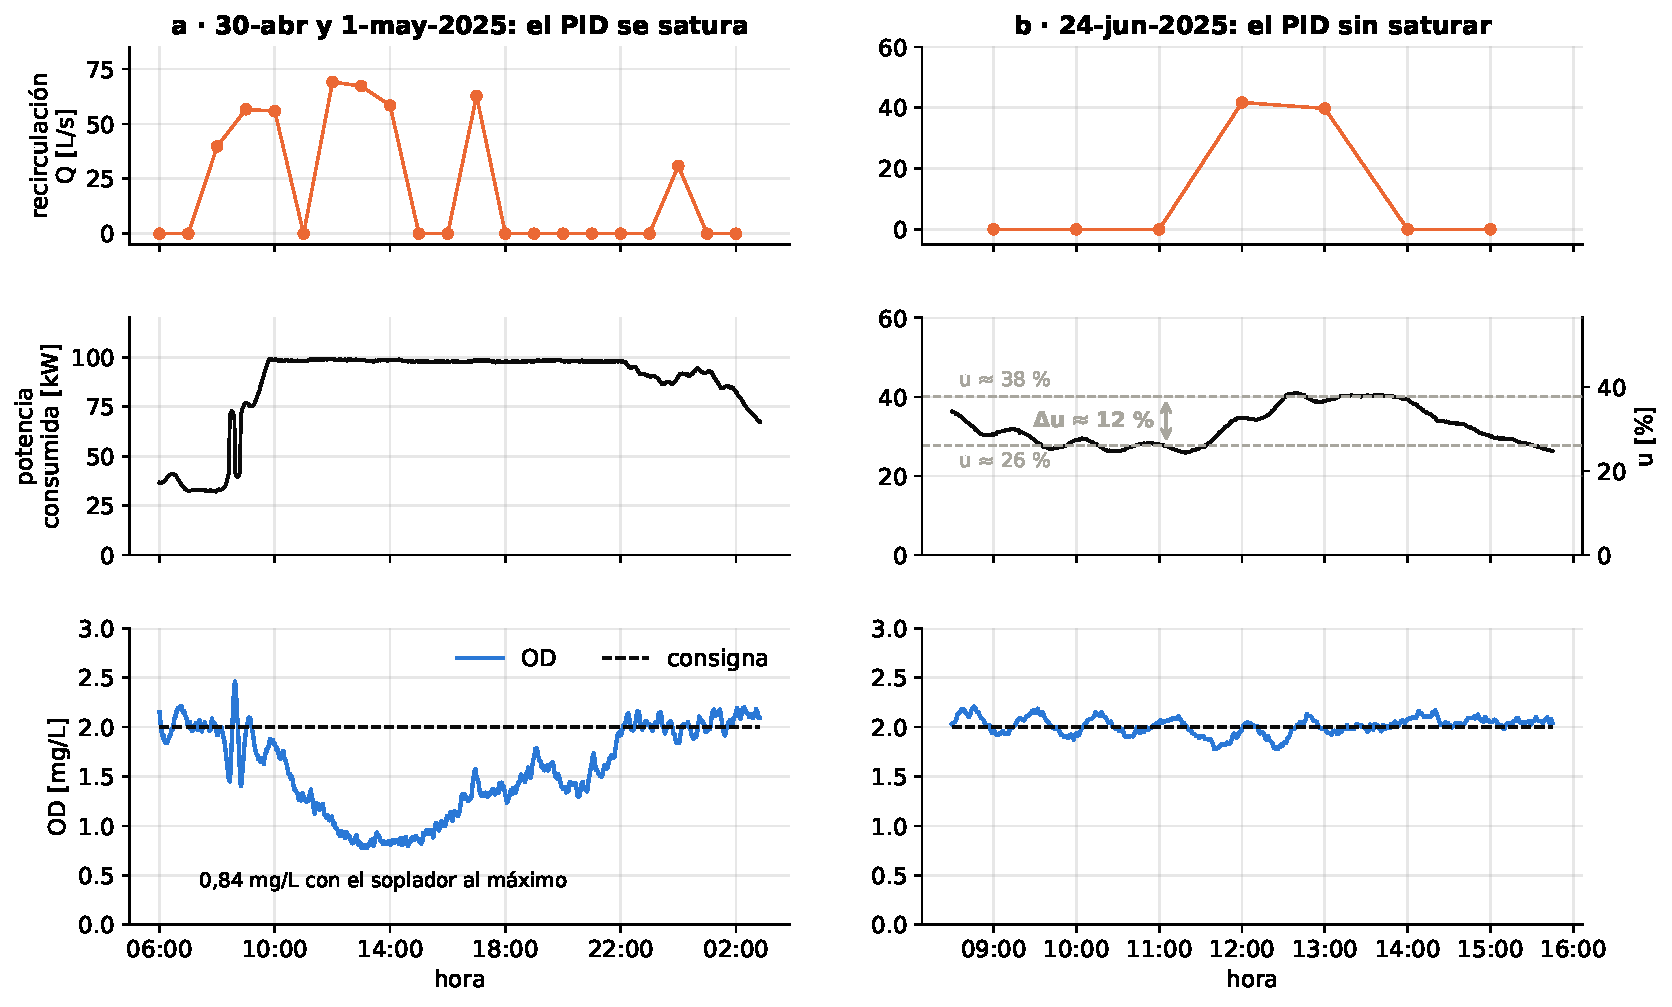
\includegraphics[width=\linewidth]{ident_23_recirculacion.pdf}
    \caption[Recirculación de lodos en M2]{Recirculación de lodos en M2 con el PID
    en la consigna de 2,0~mg/L: (a) el PID se satura; (b) sin saturarlo, con la señal de control
    equivalente $u = 100\,P/P_{\max}$ en el eje derecho de la potencia. Las gráficas muestran:
    caudal de recirculación (FIT-102), con un registro por hora; potencia consumida; OD.}
    \label{fig:ident_recirculacion}
\end{figure}



% ----------------------------------------------------------------------------
\subsection{Perturbación total medida}
\label{sec:ident_perturbacion}

Si bien para sintonizar los controladores no es necesario conocer la
perturbación completa, sí se puede usar para simularlos y para sintonizar el
observador. Por ende, la perturbación total $\bar{\xi}$ de $\dot y = \bar{\xi} + \bo u$ se
saca de los datos de M2, despejándola de esa misma ecuación, con la derivada del OD
aproximada por la diferencia centrada:
\begin{equation}
\bar{\xi}[k] = \frac{y[k+1] - y[k-1]}{2\,T_s} - \bo\,u[k-1],
\label{eq:ident_xi_medida}
\end{equation}
con $T_s = 1$~min, $y$ el OD medido, $u = 100\,P/P_{\max}$ la señal de control
equivalente (Sección~\ref{sec:ident}) y el $\bo$ de diseño, $0{,}15$~mg/(L$\cdot$h$\cdot$\%);
$u$ entra con una muestra de atraso por el retardo. La diferencia centrada es el promedio de
la diferencia hacia adelante, $(y[k+1]-y[k])/T_s$, y la de hacia atrás; sin agregar ningún otro
filtro, reduce casi a la mitad los saltos entre minutos frente a la primera. Así, $\bar{\xi}$ es una
señal medida, sin modelo: todo lo que mueve el OD sin depender de $u$.

Se calcula en los días limpios de M2, con el registro completo, el OD entre 0,3 y 5~mg/L y el
soplador sin quedarse saturado ni apagado: quedan 57 días, 52 con el PID y 5 en manual. En ellos,
$\bar{\xi}$ es negativa, porque la biomasa consume oxígeno, y además los caudales de entrada y de
recirculación mueven el OD \eqref{ecu:disturbance}; su nivel y su variación se guardan en la
Tabla~\ref{tab:ident_resumen}. El ruido de la sonda no se suma a $\bar{\xi}$, sino a la salida
simulada (Sección~\ref{sec:ident_ruido}).

La Figura~\ref{fig:ident_perturbacion} muestra el tramo que se usa en las simulaciones del
Capítulo~\ref{cap:comparacion_pid}. Al principio el soplador no se satura; de la hora 1,5 a la 6
se queda en el máximo que tenía en ese momento (en automático, en algunos casos los operarios no
dejaban que los motores llegaran al 100~\%, por eso aquí se satura antes), porque $\bar{\xi}$ queda
por debajo de lo que el soplador alcanza a compensar, y el OD cae.

\begin{figure}[H]
    \centering
    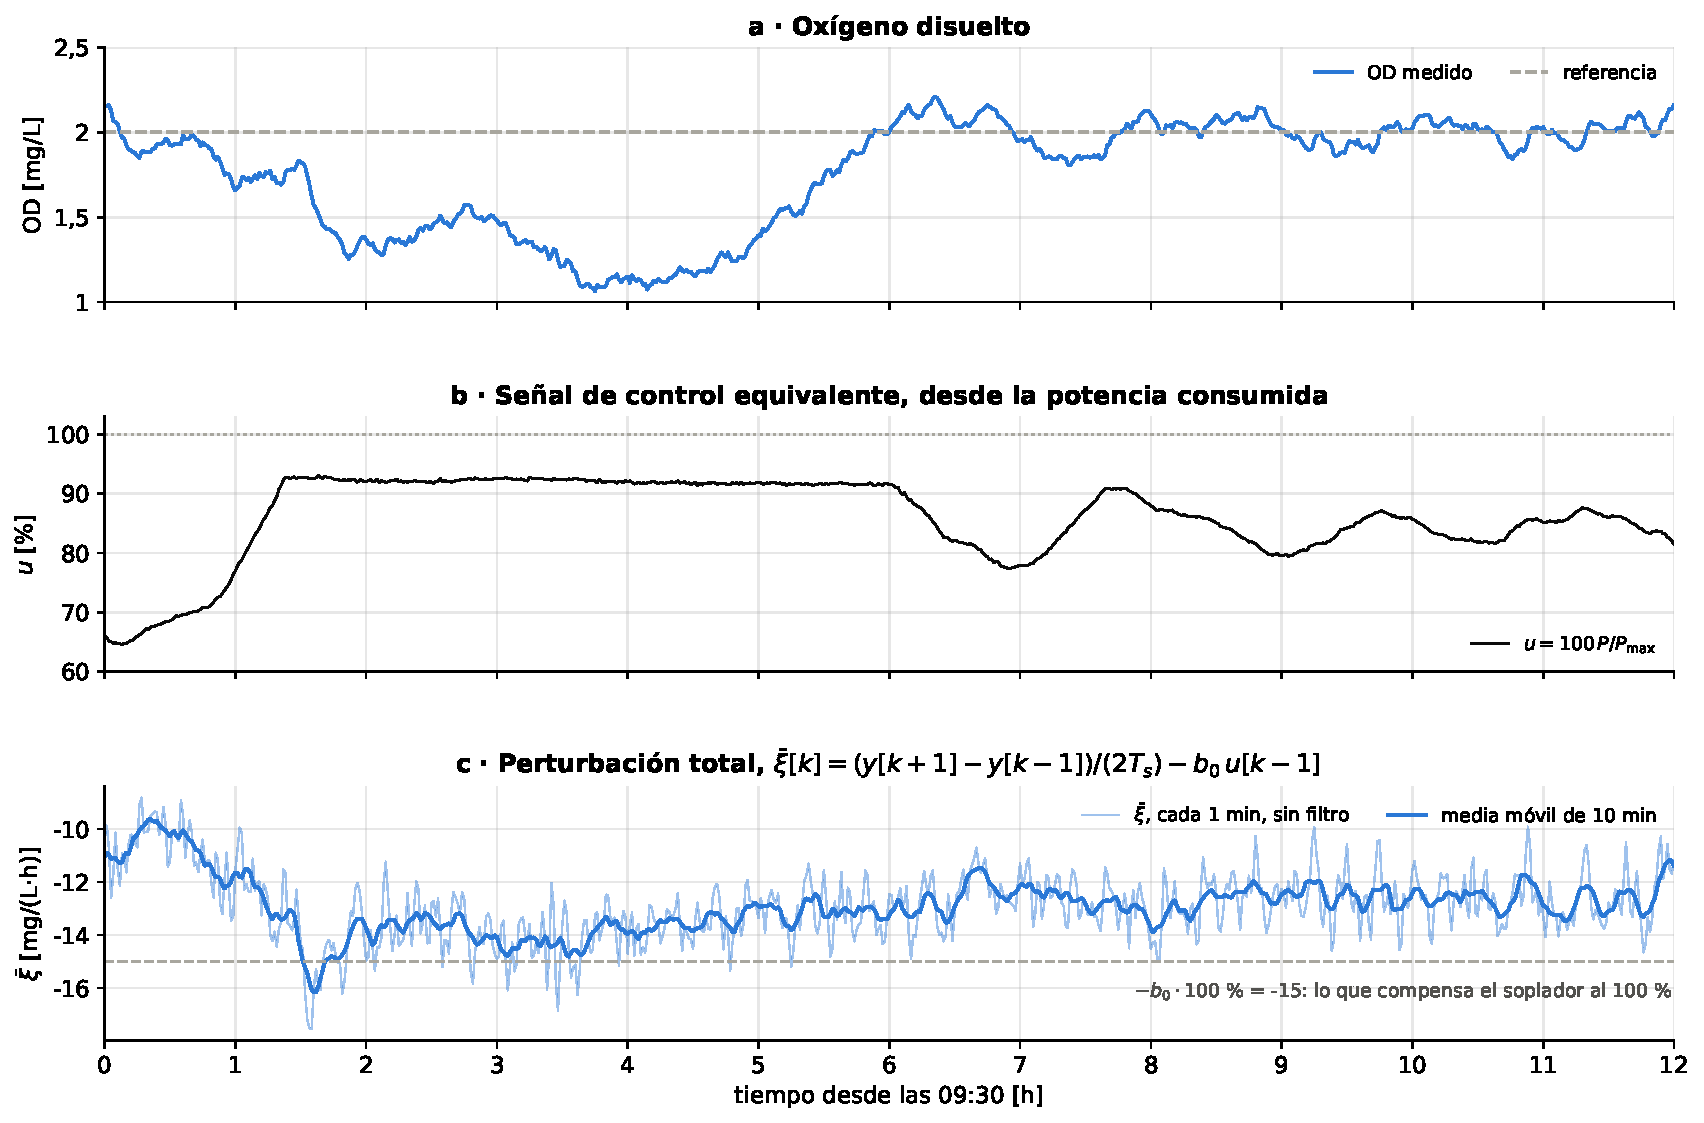
\includegraphics[width=0.85\linewidth]{ident_17_perturbacion.pdf}
    \caption[La perturbación total medida]{Perturbación total medida en M2, 12~h a 1~min:
    (a) OD medido y referencia; (b) señal de control equivalente; (c) $\bar{\xi}$ de
    \eqref{eq:ident_xi_medida}, sin filtro y con una media móvil de 10~min solo para la
    visualización. La línea discontinua de (c), $-\bo \cdot 100~\%$, es lo que compensa el
    soplador al 100~\%.}
    \label{fig:ident_perturbacion}
\end{figure}



% ----------------------------------------------------------------------------
\subsection{Espectro de la perturbación total}
\label{sec:ident_espectro}
El observador del ADRC tiene que seguir a $\bar{\xi}$, así que su ancho de banda $\wo$ debe quedar por
encima de las frecuencias donde $\bar{\xi}$ tiene la mayor parte de su energía. Para verlo se calculó, con el
método de Welch, el espectro de $\bar{\xi}$ en cada día limpio completo (un segmento de $N = 1440$~min,
un día, con ventana de Hann) y se promediaron los 54 días, con la frecuencia en rad/h, las unidades de
$\wo$ (Figura~\ref{fig:ident_espectro_f}a), y la fracción de la energía acumulada hasta $\omega_k$,
\begin{equation}
E(\omega_k) = 100~\% \cdot \frac{\sum_{i=0}^{k} P[i]}{\sum_{i=0}^{N/2} P[i]},
\label{eq:ident_energia}
\end{equation}
con $P[i]$ la densidad espectral; la frecuencia donde $E$ cruza el 50, 90 y 99~\% se guarda en la
Tabla~\ref{tab:ident_resumen}.

\begin{figure}[!htbp]
    \centering
    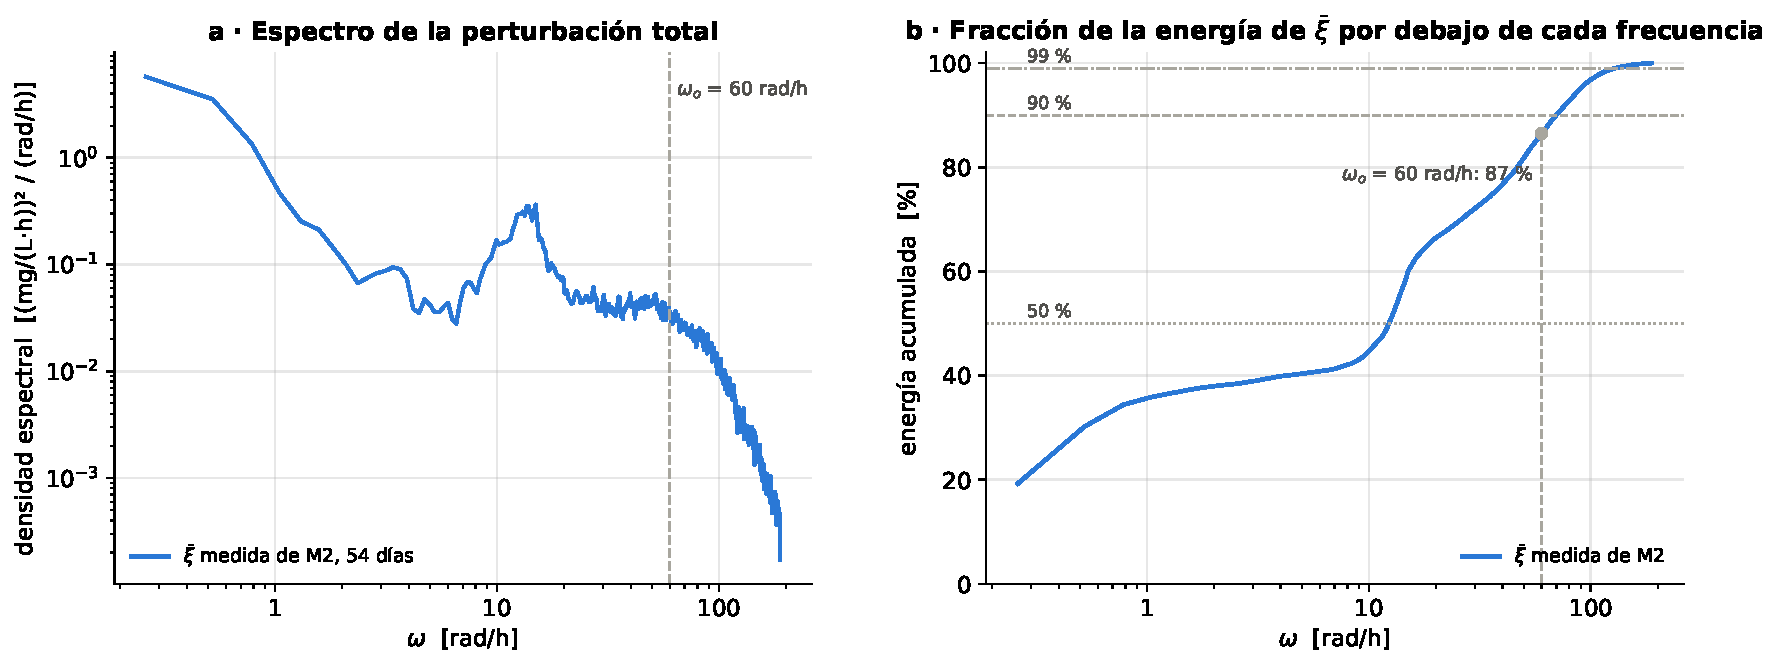
\includegraphics[width=\linewidth]{ident_19_espectro_f.pdf}
    \caption[Espectro de la perturbación total]{Espectro de la perturbación
    total medida en M2, promedio de 54 días: (a) densidad espectral; (b)
    fracción de la energía de $\bar{\xi}$ que queda por debajo de cada frecuencia, con el
    $\wo$ de diseño.}
    \label{fig:ident_espectro_f}
\end{figure}

La perturbación medida tiene energía en todo el rango: el nivel y el ciclo diario a la izquierda,
un pico cerca de 14~rad/h, que es la oscilación del PID de la planta (también está en $u$ y en el
OD), y la variación de minuto a minuto, hasta el límite del muestreo. Con el $\wo$ de diseño,
60~rad/h (Sección~\ref{subsec:caso_parametros}), el observador sigue el 87~\% de la energía de
$\bar{\xi}$; el resto es esa variación de minuto a minuto, que no conviene perseguir. El límite
superior de $\wo$ no lo pone la perturbación, sino el ruido de la medida y el retardo del lazo, y
se trata en el diseño del observador.

% ----------------------------------------------------------------------------
\subsection{Ruido del sensor}
\label{sec:ident_ruido}

El ruido del sensor de OD se midió con una sola medida: la traza del PLC
a 50~ms del ensayo del 12 de marzo de 2026 en M1. Se usan los últimos
10~min del escalón, con la consigna del soplador fija en 95~\% y el OD cerca de
su estacionario (Figura~\ref{fig:ident_ruido}), se usa la medida del oxígeno promedio entre los dos transmisores AIT-100-A y AIT-100-B, calculado por el PLC.
El estimador es $\sigma = \mathrm{std}(\Delta y)/\sqrt{2}$, que supone ruido
blanco. A 50~ms el ruido del promedio de ambos sensores es de 0,0011~mg/L. La
densidad espectral de esos 10~min (Figura~\ref{fig:ident_ruido}b) confirma
la hipótesis: desde unos 2000~rad/h hasta la frecuencia de Nyquist tiene un
piso plano, al nivel de un ruido blanco de esa $\sigma$; por debajo domina la
variación real del OD.

Para M2 y M3 no hay trazas a 50~ms, así que su valor sale del SCADA a 1~min
(Tabla~\ref{tab:ident_ruido}). A esa resolución el mismo estimador ya no mide
ruido del sensor sino la variación del OD de un minuto a otro: la misma traza
del 12 de marzo, promediada a 1~min, da 0,024~mg/L, igual que el valor del
SCADA para M1 (0,024). El valor de M3, unas 19 veces mayor que el de M1 y 14 veces mayor que
el de M2 con la misma planta y la misma aireación, apunta a un problema de su
sonda.


\begin{table}[!htbp]
\centering
\caption{Ruido del OD por módulo, $\sigma = \mathrm{std}(\Delta y)/\sqrt{2}$.
En el SCADA se descarta el 1~\% de los saltos más grandes.}
\label{tab:ident_ruido}
\small
\begin{tabular}{lllr}
\toprule
\textbf{Módulo} & \textbf{Fuente} & \textbf{Muestreo} & \textbf{$\sigma$ [mg/L]} \\
\midrule
M1 & PLC ctrlX (ensayo del 12-mar-2026) & 50~ms & 0,0011 \\
M2 & SCADA (historiador) & 1~min & 0,0326 \\
M3 & SCADA (historiador) & 1~min & 0,4589 \\
M1 (referencia) & SCADA (historiador) & 1~min & 0,0242 \\
\bottomrule
\end{tabular}
\end{table}

\begin{figure}[!htbp]
    \centering
    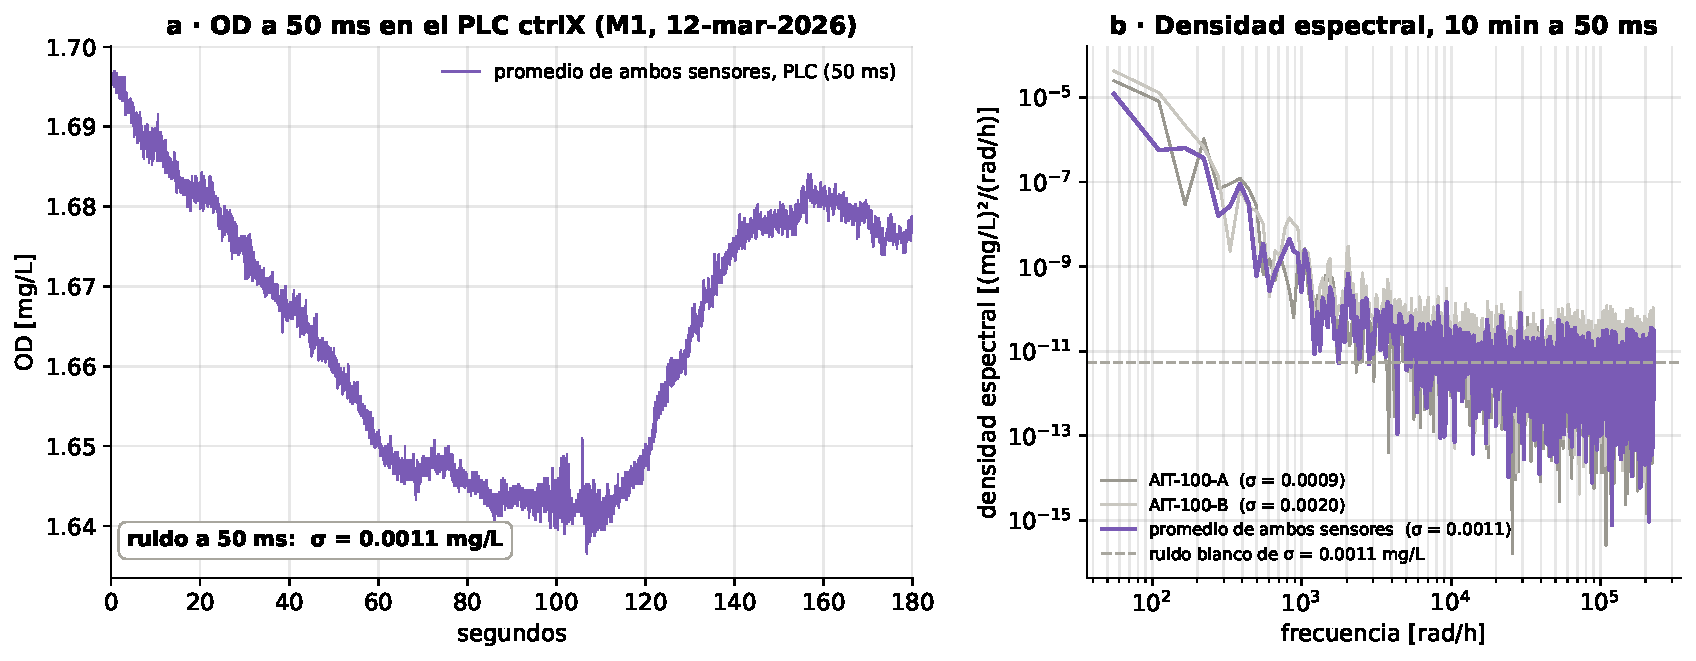
\includegraphics[width=\linewidth]{ident_18_ruido_ctrlx.pdf}
    \caption[Ruido del sensor medido a 50 ms]{Ruido del sensor de OD medido con
    el PLC ctrlX en M1, en el ensayo del 12 de marzo de 2026. (a) Tres minutos
    del promedio de ambos sensores a 50~ms con su $\sigma$. (b) Densidad
    espectral de los últimos 10~min, de cada sensor y de su promedio, con el
    nivel de un ruido blanco de la misma $\sigma$.}
    \label{fig:ident_ruido}
\end{figure}

% ----------------------------------------------------------------------------
\subsection{Planta nominal}
\label{sec:ident_planta_diseno}

Los controladores se diseñan sobre una sola planta nominal: el primer orden y con
retardo como parámetro de validación, Ecuación~\eqref{eq:ident_planta_diseno} con $k_{dc} = 0{,}05$~mg/(L$\cdot$\%),
$\tau = 20$~min y $\theta = 50$~s, es decir,

\begin{equation}
G_p(s) = \frac{0{,}05}{1200\,s + 1}\,e^{-50\,s},
\label{eq:ident_planta_diseno}
\end{equation}

o, en la forma de cadena de integradores del ADRC \eqref{eq:car_b0}, donde $\theta$ no se toma para el
diseño, pero sí para validar la robustez del sistema, con los márgenes de fase y de ganancia, y verificar
que pueda sostener este retardo.

Para que un mismo controlador sirva en los dos módulos, se toma
$k_{dc} = 0{,}05$~mg/(L$\cdot$\%), que queda entre los escalones de M2 y
los de M3 (Figura~\ref{fig:ident_validacion}), y $\tau = 20$~min, cerca de la
mediana de los escalones. Con ellos, el controlador usa
$\bo = k_{dc}/\tau = 0{,}15$~mg/(L$\cdot$h$\cdot$\%), es decir,
$4{,}17\times10^{-5}$~mg/(L$\cdot$s$\cdot$\%). Para revisar la robustez, la
ganancia se varía a través de $b_0$: el barrido del $b_0$ del controlador de la
Sección~\ref{subsec:caso_variacion}, de $1/6$ a $6$ veces el de diseño, abarca el rango
intercuartílico de $b_0$ de los dos módulos (Tabla~\ref{tab:ident_arx}), que va de $0{,}22$ a $1{,}5$
veces el de diseño. Además, $\tau$ se varía en los rangos intercuartílicos de M2 y M3, entre $11$
y $40$~min, y $\theta$ entre $0$ y $60$~s (Sección~\ref{sec:ident_retardo}). La Figura~\ref{fig:ident_planta_diseno}
muestra la respuesta de la planta nominal a un escalón de 0 a 40~\% en $u$, el
que sostiene los $2{,}0$~mg/L.

\begin{figure}[!htbp]
    \centering
    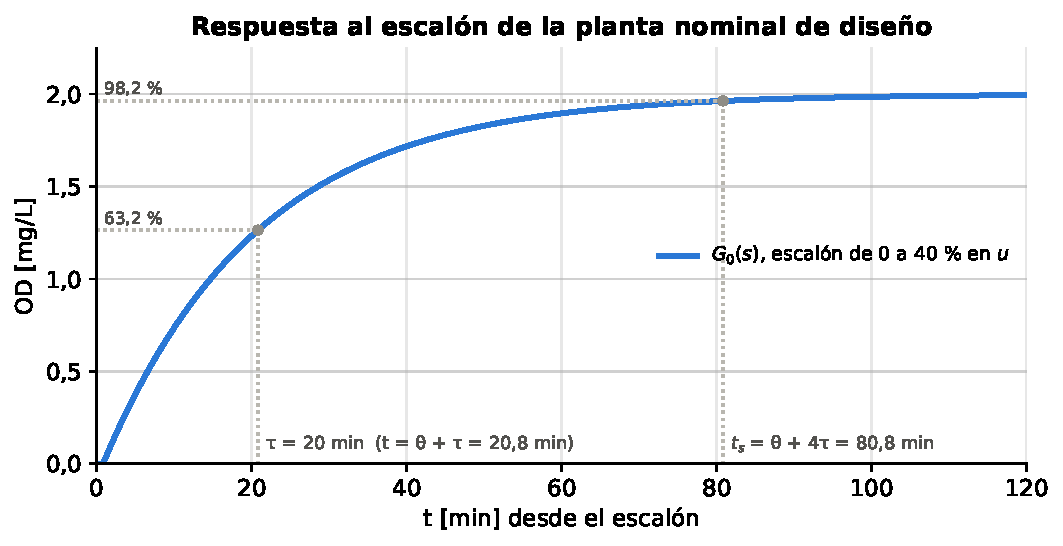
\includegraphics[width=0.85\linewidth]{ident_20_planta_diseno.pdf}
    \caption[Respuesta al escalón de la planta nominal de diseño]{Respuesta de
    la planta nominal de diseño \eqref{eq:ident_planta_diseno} a un escalón de
    0 a 40~\% en la señal de control. Las líneas punteadas grises marcan la
    constante de tiempo (63,2~\% del cambio) y el tiempo de asentamiento,
    $t_s = \theta + 4\,\tau$ (98,2~\% del cambio).}
    \label{fig:ident_planta_diseno}
\end{figure}

% ----------------------------------------------------------------------------
\subsection{Resumen de los parámetros identificados}
\label{sec:ident_resumen}

La Tabla~\ref{tab:ident_resumen} reúne los rangos de todo lo caracterizado en
esta sección: la dinámica de la planta para M2 y M3, con todas las ventanas
ARX, y la planta nominal de diseño, común a los dos módulos. Para la ganancia, el
rango que se usa en el diseño es el de $b_0$: de $0{,}0335$ a $0{,}224$~mg/(L$\cdot$h$\cdot$\%)
entre los dos módulos, es decir, de $0{,}22$ a $1{,}5$ veces el $b_0$ de diseño. Ahora bien, el
retardo, entre 0 y 60~s, es pequeño frente a
esa dinámica. Por ende, el controlador tiene que funcionar en todos estos
rangos con una sola sintonía, que es justamente lo que se busca con el ADRC.
Además, el espectro de la perturbación medida indica que la mayor parte de su energía
(87~\%) está por debajo de 60~rad/h, el ancho de banda del observador $\wo$; el resto es
variación de minuto a minuto, y el máximo de $\wo$ lo ponen el ruido de la medida y el retardo.

\begin{table}[!htbp]
\centering
\caption{Resumen de la caracterización. La dinámica de la planta se da para
M2 y M3; el resto, para M2.}
\label{tab:ident_resumen}
\footnotesize
\renewcommand{\arraystretch}{1.0}
\begin{tabular}{llc}
\toprule
\textbf{Magnitud} & \textbf{Condición} & \textbf{Rango} \\
\midrule
\multicolumn{3}{l}{\emph{Dinámica de la planta, M2}} \\
$K$ [mg/(L$\cdot$\%)] & todas las ventanas, rango intercuartílico & 0,0077 -- 0,0342 \\
$\tau$ [min] & todas las ventanas, rango intercuartílico & 11 -- 26 \\
$\bo$ [mg/(L$\cdot$h$\cdot$\%)] & todas las ventanas, rango intercuartílico & 0,0335 -- 0,107 \\
\midrule
\multicolumn{3}{l}{\emph{Dinámica de la planta, M3}} \\
$K$ [mg/(L$\cdot$\%)] & todas las ventanas, rango intercuartílico & 0,0212 -- 0,109 \\
$\tau$ [min] & todas las ventanas, rango intercuartílico & 15 -- 40 \\
$\bo$ [mg/(L$\cdot$h$\cdot$\%)] & todas las ventanas, rango intercuartílico & 0,0816 -- 0,224 \\
\midrule
\multicolumn{3}{l}{\emph{Planta nominal de diseño (M2 y M3)}} \\
$k_{dc}$ [mg/(L$\cdot$\%)] / $\tau$ [min] / $\theta$ [s] & planta nominal (Sección~\ref{sec:ident_planta_diseno}) & 0,05 / 20 / 50 \\
$\bo$ de diseño [mg/(L$\cdot$h$\cdot$\%)] & $k_{dc}/\tau$ & 0,15 \\
\midrule
\multicolumn{3}{l}{\emph{Retardo}} \\
$\theta$ [s] & rango de diseño (medido en M1: 39 y 50~s el ideal) & 0 -- 60 \\
\midrule
\multicolumn{3}{l}{\emph{Ruido del sensor} [mg/L]} \\
$\sigma$ del OD promedio & traza del PLC a 50~ms, M1 & 0,0011 \\
\midrule
\multicolumn{3}{l}{\emph{Caudal de entrada de M2} [L/s]} \\
Entrada (FIT-101) & media / variación del ciclo diario & 34 / 9,4 \\
\quad desviación respecto al ciclo & $\sigma$, robusta & 13,6 \\
\midrule
\multicolumn{3}{l}{\emph{Perturbación total medida} [mg/(L$\cdot$h)]} \\
Media & 57 días limpios & $-7{,}49$ \\
Desviación & $\sigma$, robusta & 4,05 \\
Cambio entre minutos & mediana / percentil 95 & 0,60 / 2,06 \\
\midrule
\multicolumn{3}{l}{\emph{Espectro de $\bar{\xi}$} [rad/h]} \\
50~\% de la energía & por debajo de & 12,6 \\
90~\% de la energía & por debajo de & 70 \\
99~\% de la energía & por debajo de & 129 \\
Energía por debajo de $\wo = 60$~rad/h & fracción del total & 87~\% \\
\bottomrule
\end{tabular}
\end{table}
